\documentclass[../../main.tex]{subfiles}

% 

\begin{document}
\chapter{Spektroskopie neutronů}

\section{Interakce neutronů}

Jelikož neutrony nemají elektrický náboj, při průchodu látkou neinteragují Coulombickou interakcí (což dominovalo v energetických ztrátách u nabitých částic). Neutrony interagují pouze silnou interakcí. Neutrony samy neionizují (jedná se o záření nepřímo ionizující). Neutron má magnetický moment, tudíž může interagovat i elektromagneticky, většinou to má ale zanedbatelný vliv. Neutrony tak mohou procestovat několik centimetrů látky bez jakékoliv interakce, a být tak zcela nezaznamenatelnými pro běžné detektory. Pakliže neutron interaguje, jedná se o interakci s jádrem absorbujícího materiálu. Výsledkem této interakce může být \quotedblbase zmizení\textquotedblright ~neutronu a jeho \quotedblbase nahrazení\textquotedblright ~sekundárním zářením (například ionizaci prostředí způsobují až sekundární částice, jež vznikají při interakci neutronů s jádry atomů - jsou jimi např. odražená lehká jádra, záření $\gamma$, protony, částice $\alpha$), či značná změna energie a směru letu neutronu. 

Rozdělení neutronů podle jejich energie:
\begin{itemize}
	\item Ultrachladné: $E < 10^{-6} ~\mathrm{eV}$
	\item Chladné a velmi chladné: $E = (10^{-6} ~\mathrm{eV} - 0,005 ~\mathrm{eV})$
	\item Tepelné neutrony - ($0,002 ~\mathrm{eV} - 0,5 ~\mathrm{eV}$) neutrony v tepelné rovnováze s okolím, Maxwellovo rozdělení rychlostí pro $20^ \circ C$ je nejpravděpodobnější rychlost $v = 2200 ~\mathrm{m/s}$ $\rightarrow E = 0,0253 ~\mathrm{eV}$
	\begin{equation}
	\dfrac{dN}{dv} = \dfrac{4 N}{v_{0}^3 {\pi}} v^2 \exp (- v/v_0)^2
	\end{equation}
	\begin{equation}
	\sigma (v) = \sigma_0 \dfrac{v_0}{v}
	\end{equation}
	\item Experimentální neutrony a rezonanční neutrony: $E = (0,5 ~\mathrm{eV} - 1000 ~\mathrm{eV})$
	\item Kadmiový práh: $\sim 0,5 ~\mathrm{eV}$ - s větší energií procházejí $1 ~\mathrm{mm}$ Cd
	\item Pomalé neutrony: $E < 1 ~\mathrm{keV}$
	\item Neutrony středních energií: $E = (1 ~\mathrm{keV} - 500 ~\mathrm{keV})$
	\item Rychlé neutrony: $E = (0,5 ~\mathrm{MeV} - 20 ~\mathrm{MeV})$
	\item Neutrony vysokých energií: $E = (20 ~\mathrm{MeV} - 100 ~\mathrm{MeV})$
	\item Relativistické neutrony: $E = (0,1 ~\mathrm{GeV} - 10 ~\mathrm{GeV})$
	\item Ultrarelativistické neutrony: $E > 10 ~\mathrm{GeV}$
\end{itemize} 
$\Rightarrow$ různé typy detektorů a reakcí.

Neutrony po vstupu do látky interagují téměř výhradně s atomovými jádry, a to těmito způsoby:
\begin{itemize}
	\item pružným rozptylem (ozn. ($n,n$), účinný průřez $\sigma _{n,n}$)
	\item nepružným rozptylem (ozn. ($n,n'$), $\sigma_{n,n'}$)
	\item jadernými reakcemi s emisí nabité částice (ozn. ($n,\alpha$), ($n,p$), $\sigma_{n,\alpha}$, $\sigma_{n,p}$)
	\item radiační záchyt neutronu (ozn. ($n,\gamma$), $\sigma_{n,\gamma}$)
	\item štěpením jádra (ozn. ($n,f$), $\sigma_{n,f}$, kde $f$ je produkt štěpení(fission product))
	\item tříštivé reakce, hadronová sprška
\end{itemize}
Sekundární částice produkované při neutronových interakcích, na rozdíl od $\gamma$ záření, jsou téměř vždy těžké nabité částice. Jsou produkovány buď  jako výsledek neutronem indukovaných jaderných reakcí, anebo mohou být samy jádry absorbátoru, které získaly srážkou energii. Většina neutronových detektorů používá některý z těchto typů konverze neutronu v sekundární nabité částice, které lze pak přímo detekovat. Relativní pravděpodobnosti různých druhů neutronových interakcí se dramaticky mění s energií neutronu - proto zjednodušeně dělíme neutrony na \quotedblbase pomalé\textquotedblright ~neutrony a \quotedblbase rychlé\textquotedblright ~neutrony. Pro nízkoenergetické neutrony se potom využívá neutronová difrakce.

\subsection{Interakce pomalých neutronů}

Významné interakce pro tyto neutrony jsou pružný rozptyl na jádrech absorbátoru a velké množství neutrony indukovaných reakcí. Vzhledem k malé energii nesené neutronem, pouze nepatrné množství energie se při elastickém rozptylu přenáší na jádro - tímto typem interakce tudíž nelze pomalé neutrony detekovat. Pružný rozptyl ovšem často slouží k dovedení pomalých neutronů do tepelné rovnováhy s okolním materiálem.

Teprve neutrony indukované jaderné reakce, při kterých vznikají sekundární částice záření o dostatečné energii k detekci, jsou v praxi důležité. Jelikož energie neutronu je velmi nízká, všechny tyto reakce musejí mít kladnou hodnotu $Q$, aby byly energeticky možné. Ve většině materiálů hraje při zeslabení svazku neutronů, či při neutronovém stínění nejdůležitější roli radiační záchyt ($n, \gamma$), který může sloužit i pro neupřímnou detekci neutronů za použití aktivačních fólií. Přijatelnější pro detekci jsou ale reakce ($n,\alpha$), ($n,p$) anebo ($n$, štěpení) díky tomu, že jako sekundární částice vznikají nabité částice.

\subsection{Interakce rychlých neutronů}

Pravděpodobnost většiny neutrony indukovaných reakcí, které lze potenciálně využít k detekci, rapidně klesá s rostoucí energií neutronů. Naopak rozptyl se stává důležitějším díky tomu, že odražená jádra v tomto případě dostala hodně energie umožňující snadnou detekci (neutron současně při každé srážce ztrácí energii a je moderován na nižší energie). Nejefektivnější moderátor je vodík, neboť při jedné srážce s ním může neutron ztratit až celou svou energii; pro těžší jádra je možný jen částečný přenos energie.

Pokud má neutron dostatečně velkou energii, může dojít k nepružnému rozptylu na jádře, které je tak excitováno na některou z vyšších hladin. Při deexcitaci je následně vyzářen foton. Neutron navíc při tomto procesu ztrácí větší část své energie, než by ztratil při ekvivalentním pružném rozptylu. Nepružný rozptyl a následné $\gamma$-záření hraje důležitou roli ve stínění vysokoenergetických neutronů, ale je nevítanou komplikací v odezvě mnoha detektorů rychlých neutronů založených na pružném rozptylu.

\subsection{Pružný rozptyl}

Pružný rozptyl neutronů na jádrech je nejčastějším způsobem interakce rychlých neutronů při jejich průchodu látkovým prostředím, zvláště s lehkými jádry. Proces probíhá tak, že letící neutron narazí na jádro, předá mu část své kinetické energie, odrazí se od něj a pokračuje v pohybu ve změněném směru a se sníženou energií. Odražené jádro díky svému kladnému náboji při svém pohybu vyvolává ionizaci okolních atomů, čímž ztrácí svou energii. Zpomalování je proces řady nezávislých pružných rozptylů neutronu na jádrech (pak se k detekci využívají scintilační detektory). Např. Cd má vysoké účinné průřezy pro pomalé neutrony a proto je výhodné rychlé neutrony zpomalovat. Využití odraženého jádra při rozptylu je k určení energie neutronu. 

Při pružném rozptylu se nemění kinetická energie, platí zákon zachování kinetické i celkové energie. 

\begin{itemize}
	\item Maximální předaná energie (nerelativistický případ čelní srážky) - pro neutrony s energií do $10 ~\mathrm{MeV}$:
	\begin{itemize}
		\item ZZH: $p_{n_0} = p_A - p_n$
		\item ZZE: $E_{n_0}^{KIN} = E_{A}^{KIN} \Rightarrow \dfrac{p_{n_0}^{2}}{2 m_n} = \dfrac{p_{A}^{2}}{2 m_A} + \dfrac{p_{n}^{2}}{2 m_n}$
		\item ZZH: $p_{n}^{2} = p_{A}^{2} - 2 p_A p_{n_0} + p_{n_0}^2 \Rightarrow m_A p_{n}^2 = m_A p_{A}^2 - 2 m_A p_A p_{n_0} + m_A p_{n_0}^2$
		\item ZZE: $m_A p_{n}^2 = - m_n p_{A}^2 + m_A p_{n_0}^2$
	\end{itemize}	
	\item Rovnice odečteme:
	\begin{equation}
	0 = m_A p_{A}^2 + m_n p_{A}^2 - 2 m_A p_A p_{n_0} \Rightarrow m_A p_A + m_n p_A = 2 m_A p_{n_0}
	\end{equation}
	\item Čím těžší jádro, tím nižší energii mu může neutron předat:
	\begin{equation}
	p_A = \dfrac{2 m_A p_{n_0}}{m_A + m_n}  \Rightarrow E_A = \dfrac{4 m_A m_n E_{n_0}}{(m_A + m_n)^2} = \dfrac{4A E_{n_0}}{(A+1)^2},
	\end{equation}
	kde $A = m_A /m_n$.
\end{itemize}
Kinetická energie předaná jádru při pružném rozptylu je největší pro jádra vodíku (při jedné srážce předána téměř polovina energie) a s rostoucí hmotností (nukleonovým číslem) jader klesá - proto jsou rychlé neutrony nejvíce zpomalovány látkami obsahujícími lehké prvky. Využití vodíku ($\varTheta$ - úhel rozptylu neutronu, $\psi$ - úhel odrazu protonu) $m_p = m_n$:
\begin{itemize}
	\item $p_n = p_{n_0} \cos \varTheta \Rightarrow E_n = E_{n_0} \cos ^2 \varTheta$
	\item $p_n = p_{n_0} \sin \psi \Rightarrow E_n = E_{n_0} \sin ^2 \psi$
	\item $p_p = p_{n_0} \sin \varTheta \Rightarrow E_p = E_{n_0} \sin ^2 \varTheta$
	\item $p_p = p_{n_0} \cos \psi \Rightarrow E_p = E_{n_0} \cos ^2 \psi$,
	kde $\psi = \pi / (2 - \varTheta)$
\end{itemize}
Pro jádro:
\begin{equation}
E _A = \dfrac{4A E_{n_0}}{(A+1)^2} \cos^2 \psi ~~~~~ \underrightarrow{\cos \varTheta _{CM} = 1 - 2 \cos^2 \psi} ~~~~~~ E_A = \dfrac{2A E_{n_0}}{(A+1)^2} (1 - \cos \varTheta _{CM})
\end{equation}

\begin{figure}[h!]
	\begin{minipage}[c]{0.5\linewidth}
		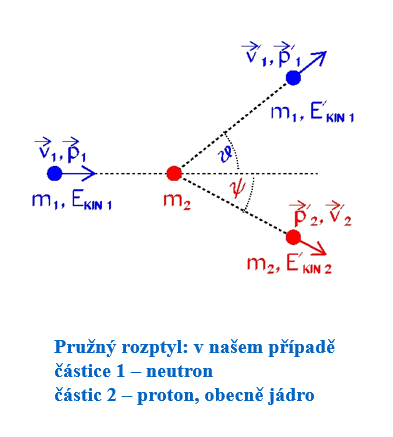
\includegraphics[width=\linewidth]{JS4_pruz1.png}
	\end{minipage}
	\hfill
	\begin{minipage}[c]{0.5\linewidth}
		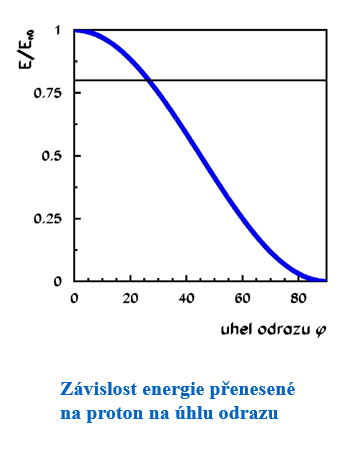
\includegraphics[width=\linewidth]{JS4_pruz2.png}
	\end{minipage}
	\caption{Pružný rozptyl}
\end{figure}

\subsection{Koherentní rozptyl - difrakce na mříži}

Nemění se velikost energie ani hybnosti a vlnové délky neutronu. Využívá se difrakce neutronů na krystalové mříži. Koherentní rozptyl je podmnožinou pružného rozptylu. Kinetická energie se v tomto případě při rozptylu nemění, terč musí být hodně těžký (hmotnost projektilu musí být oproti hmotnosti terči zanedbatelná), potom se může přenášet hybnost beze změny kinetické energie. 

Připomenutí: Braggův zákon: $n \lambda = 2d \sin \varTheta$
\begin{equation}
\lambda = \dfrac{hc}{\sqrt{2m_n c^2 E_n + E_{n}^2}} \xrightarrow{E_n << m_n c^2} \lambda = \dfrac{hc}{\sqrt{2 m_n c^2}} \dfrac{1}{\sqrt{E_n}} = 0,0288 \dfrac{1}{\sqrt{E_n}} \sqrt{\mathrm{eV}} \cdotp \mathrm{nm} ~~~\textit{pro} ~~~ E_n ~~v~~ [\mathrm{eV}]
\end{equation}

Mřížkové konstanty jsou v řádu $0,1 - 1 ~\mathrm{nm}$ $\rightarrow$ energie neutronů v řádu $\mathrm{meV}$ až $\mathrm{eV}$. 
	
\begin{center}
	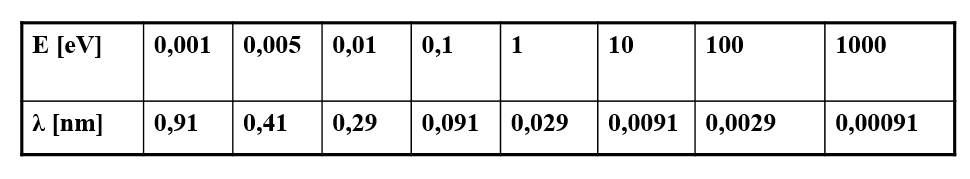
\includegraphics[width=0.9\textwidth]{JS4_koherent.png}
	\captionof{figure}{Koherentní rozptyl}		
\end{center}	

\subsection{Nepružný rozptyl}

Při nepružném rozptylu opět neutron předá část své energie jádru. Avšak v tomto případě se energie spíše než na mechanický pohyb jádra spotřebuje na zvýšení vnitřní energie jádra - nastane excitace jádra. při návratu jádra do původního stavu (deexcitaci vzbuzených jaderných hladin) se vyzáří foton záření $\gamma$, který již vyvolává ionizaci mechanismy popsanými dříve. Je to konkurenční proces k pružnému rozptylu na jádrech těžších než proton. Část energie se přemění na excitační $\rightarrow$ přesnost určení energie je dána jejím osudem. Podíl nepružného rozptylu roste s rostoucí energií.     

\subsection{Radiační záchyt neutronů ($n, \gamma$)}

Radiační záchyt je proces, při kterém je neutron jádrem pohlcen a následně je emitován jeden nebo více fotonů záření $\gamma$. To pak již samo vyvolává ionizaci. Další ionizace pak může nastat i následně dlouhodobě - jádra, jež pohltila neutron, jsou často radioaktivní a rozpadají se za vyzáření dalšího ionizujícího záření.

Radiační záchyt neutronů je nejúčinější pro pomalé neutrony s nízkou energií, zvláště pro \quotedblbase tepelné\textquotedblright ~neutrony (nazýváme tak pomalé neutrony, které po množství srážek má energii srovnatelnou s tepelným pohybem atomů) s energií přibližně $0,025 ~\mathrm{eV}$, a je odlišný pro různá jádra.

K látkám, které nejúčinněji zachycují neutrony, patří zvláště bor a kadmium, které se proto používají jako stínící materiál pro neutronové záření a pro regulaci neutronového toku v jaderných reaktorech.

Vysoké hodnoty účinných průřezů pro nízkoenergetické neutrony. Jsou to exotermické reakce. A uvolněná energie umožňuje detekci.

\subsection{Štěpení atomových jader}

Štěpení atomových jader lze schematicky rozepsat jako proces
\begin{equation}
^{A}_{Z}X + ^{1}_{0}n \rightarrow ^{A_1}_{Z_1}Y_1 + ^{A_2}_{Z_2}Y_2 + (2 ~ nebo ~ 3)n + 200 ~\mathrm{MeV},
\end{equation}
kde uvedená energie je vazbová energie.

Pro neutron štěpící $^{235}U$ existuje několik způsobů
\begin{equation}
^{235}_{98}U + ^{1}_{0}n \rightarrow ^{93}_{37}Rb + ^{141}_{55}Cs + 2 ^{1}_{0}n + 200 ~\mathrm{MeV}
\end{equation}
\begin{equation}
^{235}_{98}U + ^{1}_{0}n \rightarrow ^{94}_{36}Kr + ^{140}_{56}Ba 2 ^{1}_{0}n
\end{equation}
\begin{equation}
^{235}_{98}U + ^{1}_{0}n \rightarrow ^{101}_{38}Sr + ^{133}_{54}Xe  2 ^{1}_{0}n
\end{equation}
Energetické spektrum neutronů je spojité, přičemž 99 $\%$ tvoří okamžité neutrony a 1 $\%$ zpožděné neutrony (velký význam pro řízení reaktoru). Střední hodnota kinetické energie neutronů je $\left\langle E_n\right\rangle  = 1,75 ~\mathrm{MeV}$.

\textbf{Indukované štěpení: $(n,f)$}
\begin{itemize}
	\item indukováno nízkoenergetickými reakcemi (termální): $^{233}$U, $^{235}$U, $^{239}$Pu
	\item exotermické s velmi vysokým $ Q \sim 200 ~\mathrm{MeV}$
	\item indukováno rychlými neutrony: $^{238}$U, $^{237}$Np, $^{232}$Th
	\item indukováno \quotedblbase relativistickými\textquotedblright ~neutrony: $^{208}$Pb
\end{itemize}
	
\subsection{Jaderné reakce}	
	
\begin{itemize}	
	\item reakce ($n,2n$), ($n, 3n$) ... endotermické (prahové) reakce
	\item reakce $(n,d)$, ($n,t$), ($n, \alpha$), ... - reakce využívané pro detekci nízkoenergetických neutronů (exoergické): dvoučásticový rozpad složeného jádra v klidu, nerelativistické přiblížení:
	\begin{equation}
	E_j + E_c = Q
	\end{equation}
	\begin{equation}
	m_j v_j = m_c v_c ~~~~ \Rightarrow ~~~~ \sqrt{2 m_j E_j } = \sqrt{2 m_c E_c} ~~~ \Rightarrow ~~~ E_j = \dfrac{m_c}{m_j} E_c ~~~ \Rightarrow ~~~ E_c = \dfrac{m_j}{m_c + m_j} Q,
	\end{equation}
	kde $m_c, E_c$ je pro částici a $m_j, E_j$ je pro jádro.
	\item reakce využívané k detekci rychlých neutronů - prahová reakce
	\item výroba plutonia
	\item detekce tepelných neutronů: $^{10}_{5}$B$ + ^{1}_{0}n \rightarrow ^{4}_{2}\alpha + ^{7}_{3}$Li 
	\item detekce tepelných neutronů v termojaderných reakcích: $^{6}_{3}$Li$ + ^{1}_{0}n \rightarrow ^{4}_{2}\alpha + ^{3}_{1}$H 
	\item určování stáří látek organického původu
\end{itemize}	
Při vysokých energiích $E > 0,1 ~\mathrm{GeV}$ $\rightarrow$ reakce protonů a neutronů jsou podobné (de Broglieho vlnová délka je srovnatelná s velikostí nukleonu - nukleony interagují mezi sebou).

\subsection{Účinné průřezy}

Celkový účinný průřez je dán součtem, neboť jednotlivé procesy na sobě nezávisí
\begin{equation}
\sigma_t = \sigma_{n,n} + \sigma_{n,n'} + \sigma_{n,\alpha} + \sigma_{n,\gamma} + \sigma_{n,f}
\end{equation}
Pro intenzitu svazku neutronů při průchodu absorbátorem tloušťky $d$ platí vztah
\begin{equation}
I(d) = I_0 \exp (- \sigma_t n d),
\end{equation}
odkud lze odvodit vztah pro násobnost zeslabení $T = \dfrac{I_0}{I(d)} = \exp (- \sigma_t n d)$.

Dále zavádíme také makroskopický účinný průřez $\Sigma [\mathrm{m^{-1}}] = n \sigma_t$, jakožto analogii ke koeficientu zeslabení. Převrácená hodnota $l = 1 / \Sigma$ udává střední volnou dráhu (tloušťku absorbátoru, která zeslabí tok neutronů na $(1/e)$).

\subsection{Absorbční účinný průřez}

Typickou závislost $\sigma_a = \sigma_a (E_n)$ pro látky s atomovým číslem $A > 100$ znázorňuje Obr. \ref{obr:JS4_absorb}. Jak je vidno, závislost můžeme rozdělit do tří částí:
\renewcommand{\theenumi}{\Roman{enumi}}
\begin{enumerate}
	\item v první části nalézáme oblast zákona $1/v$, platí $\sigma_a = \sigma_0 \dfrac{v_0}{v}$, kde $v_0 = 2200 ~\mathrm{m \cdotp s^{-1}}$ a tedy energie $E_{n_0} = 0,025 ~\mathrm{MeV}$.
	\item $\sigma_a$ má několik maxim, jejich počet závisí na izotopu
	\item hladká funkce, blíží se geometrickému průřezu $\sigma_a = \pi R^2$, kde $R= r_0 A^{1/3}$, $r_0 = 1,45 ~\mathrm{fm}.$ 	
\end{enumerate}	
\renewcommand{\theenumi}{\arabic{enumi}}

\begin{center}
	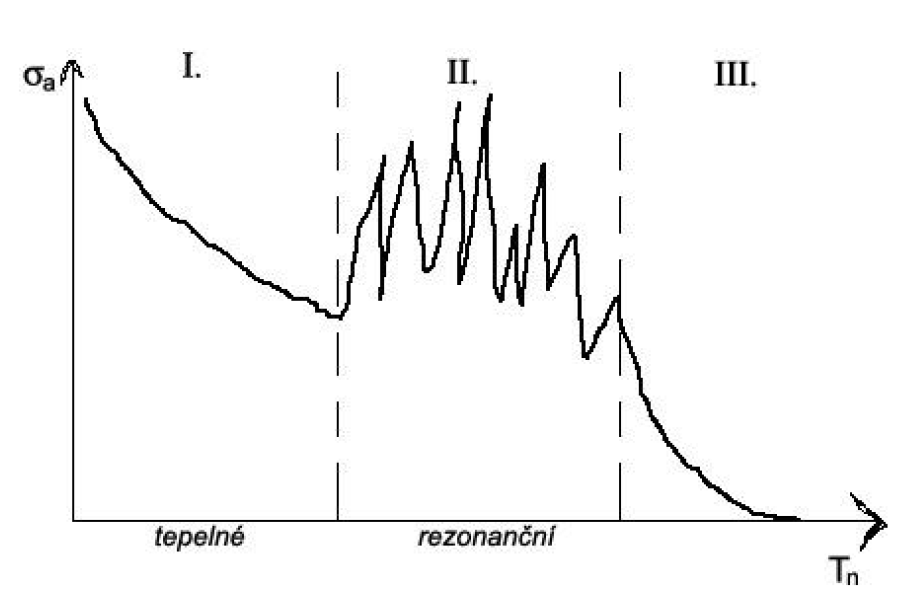
\includegraphics[width=0.7\textwidth]{JS4_absorb.png}
	\captionof{figure}{Závislost $\sigma_a$ na energii $E_n$ \label{obr:JS4_absorb}}		
\end{center}	

\subsection{Některé významné reakce s neutrony}

\begin{itemize}
	\item exotermické reakce: uvolněná energie umožňuje detekci
	\item $^{157}$Gd$(n,\gamma)$ - pro termální neutrony jeden z vůbec největších $\sigma \sim 255 000 ~\mathrm{barn}$
	\item účinný absorbátor neutronů: $^{113}_{48}$Cd$ + ^{1}_{0}n \rightarrow ^{114}_{48}$Cd$ + \gamma$
	\item radioaktivní indikátor: $^{115}_{49}$In$ + ^{1}_{0}n \rightarrow ^{116}_{49}$In$ + \gamma$, $^{116}_{49}$In$ \rightarrow ^{116}_{50}$Sn$ + e^- + \overline{\nu_e}$
	
\end{itemize}

\subsection{Tříštivé reakce, hadronová sprška}

Interagují relativistické a ultrarelativistické neutrony. Mají stejný průběh jako pro protony a  jádra.

\begin{center}
	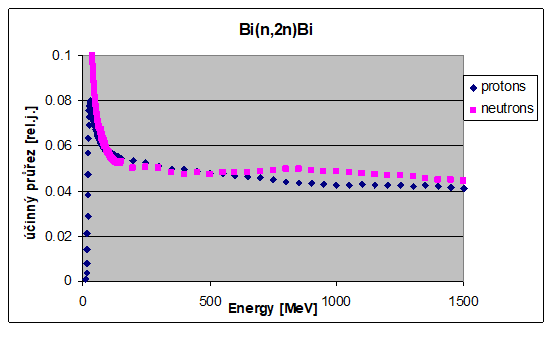
\includegraphics[width=0.7\textwidth]{JS4_hadron.png}
	\captionof{figure}{Tříštivé reakce \label{obr:JS4_hadron}}		
\end{center}

\section{Detektory a spektrometry neutronů}

Detekci neutronů rozdělujeme takto:
\begin{itemize}
	\item Detektory pomalých neutronů (tepelných, epitermálních, rezonančních)
	\item Detektory rychlých neutronů
	\item Detektory relativistických a ultrarelativistických neutronů
\end{itemize}

Detekce neutronů je prováděna skrze reakce, ve kterých se energie předává nabitým částicím nebo takové částice vznikají.

Následek:
\begin{itemize}
	\item Komplikované reakce $\rightarrow$ silná závislost účinnosti na energii
	\item Malá účinnost $\rightarrow$ nutnost velkých objemů
	\item Ztrácí jen část energie $\rightarrow$ komplikované určování energie $\rightarrow$ časté využití TOF
\end{itemize}	

Využívané reakce:
\begin{itemize}
	\item neutron + jádro $\rightarrow$ odražené jádro může být proton, deuteron, triton, $\alpha$-částice, štěpné produkty $\rightarrow$ velmi silná závislost účinného průřezu na energii
\end{itemize}

Detektory složené:
\begin{itemize}
	\item Konvertor - zajišťuje vznik nabitých částic
	\item Detektor nabitých částic
\end{itemize}

Požadavky na materiál konvertoru a detektoru:
\begin{itemize}
	\item Velký účinný průřez pro využívané reakce
	\item Vysoká uvolněná energie (pro detekci nízkoenergetických neutronů) nebo vysoká konverze kinetické energie (pro detekci vysokoenergetických neutronů)
	\item Možnost rozlišení fotonů a neutronů (nejlépe detektory citlivé k neutronům a necitlivé k $\gamma$)
	\item Co nejnižší cena na produkci materiálu
\end{itemize}

K detekci se tedy využívají:
\begin{itemize}
	\item Neutronové čítače - proporcionální čítač, konvertor (např. He) je přímo pracovní plyn nebo příměs, případně je obsažen ve stěnách (energie se pak určuje z TOF)
	\item Scintilátory - organické (odražené protony a uhlík), dopované konvertorem kapalné (NE213) nebo plastikové (NE102A)
\end{itemize}
	
\subsection{Detektory pomalých neutronů}

Musíme vybrat takový materiál, který má velký účinný průřez pro tepelné rezonanční neutrony. Důležitá je také nízká efektivita na záření $\gamma$. Využívají se exoergické reakce,  při kterých je energie uvolněná v detektoru daná energií reakce. Energii můžeme určit například z doby letu nebo difrakcí pro velmi nízkoenergetické neutrony. Pro detekci pomalých neutronů můžeme použít následující detektory:
\begin{enumerate}
	\item Detektory založené na reakci s bórem
	\begin{itemize}
		\item BF$_3$ proporcionální komora
		\begin{itemize}
			\item BF$_3$ slouží jako neutronový konvertor i jako plynná náplň proporcionálního čítače
			\item vysoké obohacení o izotop $^{10}$B
			\item nízká efektivita na záření $\gamma$
		\end{itemize}
	 \item bór na stěnách a alternativní plynová náplň 
	 \item scintilátory s obsahem bóru
	 
	 $\Rightarrow$ využití možnosti rozlišení neutronů a fotonů pomocí tvaru pulsu
	\end{itemize}
    \item Detektory založené na reakcích $^{6}$Li (dopant)
    \item Detektory založené na reakcích $^{3}$He (vždy plynná podoba) - proporcionální čítače - konvertor je zároveň náplní
    \item Detektory založené na štěpení ($^{235}$U, $^{239}$Pu)
\end{enumerate}

\subsection{Krystalové difrakční spektrometry a interferometry}	

Využití difrakce:
\begin{itemize}
	\item Určení energie neutronů
	\item Určení struktury krystalů
\end{itemize}

Využívá se ohybu krystalu pro změnu měřené energie. Monochromátory využívají odraz.

\subsection{Mechanické monochromátory $\Rightarrow$ TOF měření}

Jsou to rotující absorpční disky, které mají vhodně uspořádané otvory. Velmi přesně měří energii nízkoenergetických neutronů. Můžeme pomocí nich získávat svazky neutronů s danou energií.

\subsection{Detektory rychlých neutronů}

Rychlé neutrony se nejdříve pomocí moderátoru zpomalí na pomalé neutrony. Plastické a kapalné scintilátory umožňují zároveň detekci i moderaci. 

\begin{itemize}
	\item \textbf{Bonnerovy koule}: organický moderátor se nachází okolo neutronového detektoru tepelných neutronů
	\item spektrometrie: díky různému průměru koulí (nebo díky tomu, že se nachází v různých místech detektoru) se moderují neutrony s různou maximální energií, spektrum se rekonstruuje z naměřených četností z různě velikých koulí
	
	Odezva se simuluje pomocí Monte Carlo programů.
	
	\item Výhody: jednoduchost, široký energetický rozsah
	\item Nevýhody: velmi malé energetické rozlišení
\end{itemize}

\subsection{Detektory a spektrometry založené na pružném rozptylu neutronů}

Používají se scintilační detektory (např. NE213):
\begin{itemize}
    \item Odezva $L$: ~~~~~ $L = k \cdotp E^{3/2}$, ~~~kde $k$ je nějaká konstanta
    \item odtud dostaneme: $\dfrac{dL}{dE} = \dfrac{3}{2} k \cdotp E^{1/2}$
    \item Energie vyjádřena z odezvy: $ E = \dfrac{1}{k} L^{2/3}$
    \item Je-li: ~~~~ $\dfrac{dN}{dE} = konst.$ ~~~~ potom: ~~~~ $\dfrac{dN}{dL} = \dfrac{\dfrac{dN}{dE}}{\dfrac{dL}{dE}}= \dfrac{konst}{\dfrac{3}{2} k E^{1/2}} = konst.' \cdotp L^{-1/3}$
    
    Tyto vztahy jsou platné pro rozptyl neutronů s $E < 10 ~\mathrm{MeV}$ na protonech.
\end{itemize}
Další faktory: 
\begin{itemize}
	\item vliv okraje
	\item mnohonásobný rozptyl
	\item rozptyl na uhlíku
	\item rozlišení detektoru
	\item konkurenční reakce při větších $E_n$
\end{itemize}

\begin{center}
	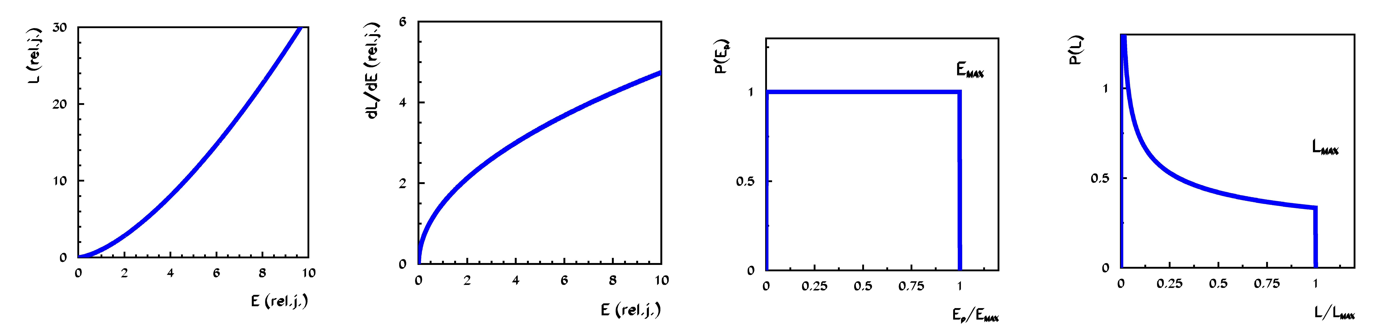
\includegraphics[width=1.05\textwidth]{JS4_spektr2.png}
	\captionof{figure}{Charakteristiky pružného rozptylu neutronů \label{obr:JS4_spektr2}}		
\end{center}

\subsection{Neutronový spektrometr založený na odražených protonech}

\begin{itemize}
	\item detekce a určení energie $E_p$ odražených protonů
	\item využití znalosti úhlu odrazu $\psi$
\end{itemize}

Existuje široká škála detektorů, které tento efekt využívají (závisí to na energii protonů, ale protony se dobře detekují, takže spíše na množství ionizace). 
Problémy:
\begin{itemize}
	\item vhodná velikost terče
	\item přesnost určení úhlu
\end{itemize}

\begin{center}
	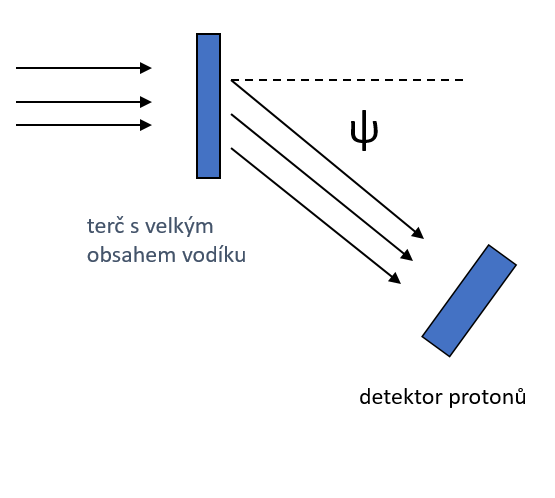
\includegraphics[width=0.5\textwidth]{JS4_spektr.png}
	\captionof{figure}{neutronový spektrometr založený na detekci odražených protonů \label{obr:JS4_spektr}}		
\end{center}

\subsection{TOF spektrometry $\Rightarrow$ měření pomocí doby letu}

Jedná se o nejpřesnější určování energie neutronů (relativistické)
\begin{equation}
E_{KIN} = E_0 \left( \dfrac{1}{\sqrt{1 - \beta^2}} - 1\right) ~~~~~~ \beta = \dfrac{v}{c} = \dfrac{L}{tc} 
\end{equation}
\begin{equation}
\sigma _{E_{KIN}} = \dfrac{\beta^2}{1 - \beta^2} (E_{KIN} + E_0 )\sqrt{\left( \dfrac{\sigma_L}{L}\right)^2 + \left( \dfrac{\sigma_t}{t}\right)^2 }
\end{equation}

Problémem je přesnost určení času interakce (interakční místo) a vzdálenosti mezi interakcí a detekcí (tloušťka detektoru).

\subsection{Aktivační detektory neutronů}

Jsou to sendviče fólií z různých materiálů (většinou monoizotopických - jinak totiž nevíme, z jaké reakce radioizotop vznikl). Využívají se různé prahové reakce, abychom mohli určit spektrum neutronů. Měří se rezonanční neutrony pro různé ($n, \gamma$) reakce (musíme dát pozor na vliv pohlcení neutronů ve fólii). Jsou zde problémy s rekonstrukcí spektra a tak musíme přímo srovnávat počty aktivovaných jader. Často se využívají zlaté fólie.

\begin{itemize}
     \item Výhody: jednoduchost, malý detektor lze vložit všude (jedná se pouze o malou fólii)
      \item Nevýhody: složitější interpretace $\Rightarrow$ účinné průřezy jsou komplikované
\end{itemize}

\subsection{Indukované štěpení a emulze}

Kombinace $^{235}$U, $^{238}$U a $ ^{208}$Pb

Počítá se počet ionizačních stop štěpných fragmentů. Jedná se ale poté o složitou analýzu a interpretaci naměřených dat.

\subsection{Detekce neutronů II}
Mechanismy detekce neutronů v látce jsou založeny na nepřímých metodách, jelikož neutrony jakožto neutrální částice neinteragují přímo s hmotou. Proces detekce neutronů je spuštěn ve chvíli, kdy tyto neutrony interagují s jádry za vzniku nabitých částic. Elektrické signály produkované těmito nabitými částicemi lze pak již detekovat.

Rozlišujeme dva hlavní druhy interakce neutronů s látkou:
\begin{itemize}
	\item \textbf{Recoil-type detector} - neutron může být rozptýlen terčovým jádrem, přičemž mu předá část své kinetické energie. Pokud je jí předáno dostatek, odražené jádro může ionizovat materiál obklopující místo interakce. Tento mechanismus je účinný pouze pro neutrony o dostatečné energii interagují s lehkými jádry. Tyto detektory zaznamenávají pouze první interakci. Celková energie neutronu povětšinou není ztracena v detektoru, tudíž jediná informace o energie je ta, zda se jednalo o nízko- či vysokoenergetický neutron, jenž byl rozptýlen.
	
	\item \textbf{Reaction-type detectors} - neutron může způsobit jadernou reakci, přičemž produkty této reakce (protony, $\alpha$ částice, $\gamma$ záření, odštěpky) mohou iniciovat proces detekce. Většina reakcí se odehrává již za tepelných energií, pouze některé mají prahovou energii. Vzhledem k tomu, že neutrony vykazují větší pravděpodobnost reakcí za tepelných energií, je v těchto typech detektorů neutrony třeba moderovat. Tím se však zcela ztrácí informace o jejich počáteční energii (energie, která je zaznamenána v detektoru, je pouze reakční energie). V těchto detektorech se používají zejména $^{3}$He při tlaku několika atmosfér, $^{6}$Li či $^{10}$B ve formě chemických sloučenin. 
\end{itemize}

\subsection{Základní parametry jednotlivých reakcí}

\begin{itemize}
	\item Reakce $^{10}$B$(n_{th}, \alpha)^{7}$Li - účinný průřez je $\sigma = 3840 ~\mathrm{b}$, $94 \%$ reakcí jde přes excitovaný stav (jenž přechází v základní stav $\gamma$- rozpadem), zbylých $6 \%$ přes základní stav, energie reakce je mnohem větší než kinetická energie tepelných neutronů, tudíž součet energie reakčních produktů je přibližně roven energii reakce ($E_{Li} = 0,84 ~\mathrm{MeV}, E_{\alpha} = 1,47 ~\mathrm{MeV}$), $^{10}$B je nejčastěji používaný materiál pro detekci tepelných neutronů.
	\item Reakce $^{6}$Li$(n_{th}, \alpha)^{3}$H - účinný průřez je  $\sigma = 940 ~\mathrm{b}$, energie reakce je mnohem větší než kinetická energie tepelných neutronů, tudíž součet energie reakčních produktů  je přibližně roven energii reakce ($E_T = 2,73 ~\mathrm{MeV}, E_{\alpha} = 2,05 ~\mathrm{MeV}$).
	\item Reakce $^{3}$He$(n,p)^{3}$H - účinný průřez je  $\sigma = 5330 ~\mathrm{b}$, energie reakce je mnohem větší než kinetická energie tepelných neutronů, tudíž součet energie reakčních produktů  je přibližně roven energii reakce ($E_p = 0,574 ~\mathrm{MeV}, E_T = 0,191 ~\mathrm{MeV}$).
\end{itemize}


Detektory používají buď mechanismus rozptylu nebo reakce, mohou používat pevné, tekuté, či plynové média. Ačkoliv výběr reakcí je omezený, můžeme obměňovat detekční média k dosáhnutí mnoha možností detekce. 

Informace o energii neutronu je většinou velmi chabá (limitována dostupnými reakcemi indukovanými neutrony). Můžeme říct, že neutronové detektory poskytují informace pouze o počtu neutronů, ale ne o jejich energii.

Po \quotedblbase konvertování\textquotedblright ~neutronů v nabité částice (díky rozptylu či jaderným reakcím) mohou být použity různé detektory částic - plynové, scintilační nebo polovodičové. Detekce neutronů se dělí na detekci tepelných, rychlých a relativistických. 

Jaderné účinné průřezy mají charakteristickou závislost na energii. Reakcím s nabitými částicemi dominuje Coulombovská energie, jelikož obě částice v reakci mají elektrický náboj. Účinný průřez tak je dán jako $\sigma (E) \sim \pi r^2 (1 - V/E)$, kde $V$ je Coulombovská bariéra. Také neutrony indukované reakce ale mají charakteristickou závislost na energii - interakce je vždy přitažlivá a účinný průřez pro záchyt s $l=0$ má tvar $\sigma _0 = 1/v$. 

Detekce neutronů převážně spoléhá na pozorování neutrony indukovaných jaderných reakcí. Účinný průřez záchytu pro reakci indukované rychlými neutrony ja malý v porovnání s tímtéž účinným průřezem při nízkých energiích neutronů ($\sigma _{cap} \sim 1/v$).

Existují dva přístupy, jak detekovat rychlé neutrony:
\begin{itemize}
	\item buď je můžeme termalizovat (moderace hydrogenními materiály jako např. polyethylenem nebo parafinem, optimální tloušťka moderátoru je v řádech $\mathrm{cm}$ čí desítkách $\mathrm{cm}$ pro energie $\mathrm{keV}$ či $\mathrm{MeV}$) a zachytit, což sice probíhá s vysokou efektivitou, ale poskytuje informace pouze o počtu neutronů, nikoliv o jejich energii, navíc je díky nutné moderaci pomalé.
	
	\item nebo je můžeme nechat se při vysokých energiích pružně rozptylovat na protonech (protony jsou lehce detekovatelné), tento přístup poskytuje rychlou odezvu a  také energetické spektrum neutronů (za předpokladu, že $E_n$ je dostatečně velké ve srovnání s $Q$); vhodné jsou reakce $^{6}$Li$(n, \alpha)$ a $^{3}$He$(n,p)$. 
\end{itemize}

Pro zpomalování rychlých neutronů se používají i tzv. \textbf{Bonnerovy sféry}. Je to organický moderátor ve tvaru koule umístěný okolo detektoru tepelných neutronů.

Neutronové detektory jsou citlivé na $\gamma$ záření, a jelikož většina materiálů emituje více než desetkrát více $\gamma$ neutronů, je citlivost na $\gamma$ významným parametrem. Na relativní výšku signálů od $\gamma$ mají vliv zejména:
\begin{itemize}
	\item přítomnost stínění před $\gamma$ zářením
	\item některé detekční materiály upřednostňují absorpci neutronů, tepelné neutrony jsou absorbovány s větší pravděpodobnostní než $\gamma$, u rychlých neutronů jsou pravděpodobnosti srovnatelné.
	\item neutrony indukují reakce, v nichž se uvolní více energie než přenese $\gamma$ elektronu (průměrná přenesená energie na jedno $\gamma$ jednomu elektronu je asi $400 ~\mathrm{keV}$). Tudíž mají elektrony v plynových detektorech mnohem delší dosah než těžké nabité částice vzniklé při reakci. Pokud je zvolena tloušťka detektoru (nebo tlak plynu) taková, aby se  v detektoru zastavily pouze těžké nabité částice, elektrony uniknou pryč a v detektoru zanechají pouze malou část své energie.
	\item rychlost sběru náboje pro neutrony a $\gamma$ se různí. Zesilovač s rychlou diferenciací tak může shromáždit relativně méně náboje z $\gamma$ interakce než z interakce neutronů. Poté lze efektivně použít diskriminaci podle tvaru pulsu. 
\end{itemize}

\subsection{Detekce založená na rozptylu neutronů}

Nejčastěji používaná metoda detekce rychlých neutronů je rozptyl na lehkých jádrech. Tato odražená jádra se následně velmi jednoduše detekují (nezajímá nás přitom hodnota energie $Q$ pružného rozptylu). 

Energie předaná jádru je závislá na jeho hmotovém čísle $A$ a je dána vztahem
\begin{equation}
E_R = \dfrac{2A}{(1+A)^2}(1 - \cos \varTheta)E_n,
\end{equation}
kde $\varTheta$ je úhel rozptylu odraženého jádra, $E_n$ je energie neutronu před srážkou. Maximální hodnota předané energie je $E_R = \dfrac{4A}{(1+A)^2}E_n. $

\subsection{Detekce založená na jaderných reakcích s neutrony}

\textbf{Štěpné neutronové komory}

Tyto detektory zaznamenávají neutrony, které indukují štěpení v štěpitelném materiálu (obvykle je jím vysoce obohacený $^{235}$U), jímž jsou obaleny vnitřní stěny komory (te je jinak plněna plynem - směsí argonu a metanu). Po štěpné reakci vzniknou dva fragmenty - jeden je absorbován ve stěně detektoru a druhý způsobí ionizaci v plynu. tato metoda je vhodná zejména pro pomalé neutrony.

\subsection{Neutronové scintilační detektory}

Ve scintilačních detektorech jsou záchytem neutronů produkovány ionty, stejně tak jsou v médiu vytvořeny krátkožijící stavy emitující fotony, které cestují ze scintilátoru k fotokatodě, kde jsou emitovány fotoelektrony. Ty jsou následně urychlovány v elektrickém poli fotonásobiče a díky dynodám je jejich počet znásoben (přibližně $10^6 $-krát), než doputují na anodu.

V těchto detektorech se používají ZnS(Ag) (obyčejně se používá ve sloučeninách s Li$_6$F), GS-20 (ve sloučenině s Li$_2$O), Li$_6$Gd(BO$_3)_3$(Ce$^{3+})$.

Pro detekci rychlých neutronů se používají plastické a organické scintilátory z důvodu jejich rychlé odezvy. Hlavní nevýhodou organických scintilátorů je však jejich vysoká citlivost na $\gamma$ záření. Pravděpodobnost detekce neutronů a $\gamma$ jsou srovnatelné, výšky pulsů pro monoenergetické záření také. Jedinou možností rozlišení typu detekované částice je ta rozlišení tvaru pulsu.

Ve scintilátorech se používá reakce
\begin{equation}
^{6}Li + n \rightarrow ^{4}He  + ^{3}H + 4,8 ~\mathrm{MeV}.
\end{equation}

\subsection{Polovodičové detektory neutronů}

V těchto detektorech se používá pro detekci neutronů výše uvedená reakce. Na každý neutron se vyprodukuje přibližně jeden a půl miliónů  elektronů a děr ($\sim 2,4 \cdotp 10^{-13} ~\mathrm{C}$). Takové množství elektrického náboje lze detekovat přímo bez dalšího zesilování.

Standardní neutronové polovodičové detektory však neobsahují dostatek jader absorbujících neutrony, aby měly rozumnou efektivitu detekce neutronů. Proto je potřeba například dávat absorbátor neutronů ($^{6}$Li) na povrch polovodiče. 

\subsection{Ostatní techniky detekce neutronů}

K detekci neutronů lze použít také mechanické zařízení, jako například rychlostního selektoru, či rotující závěrky - tyto jsou využitelné pouze v oblasti tepelných energií. Energii neutronu lze určovat prostřednictvím měření doby letu (time of flight), nebo pomocí krystalové difrakce (tepelné neutrony mají de Broglieho vlnovou délku $\sim 0,1 ~\mathrm{nm}$).

\subsection{Neutronová aktivační fólie}

Pro měření intenzity toku neutronů se používá neutronových aktivačních fólií. Jsou to čisté materiály se známou hustotou a účinným průřezem. 

Neutrony i velmi nízkých energií mohou interagovat s jádry a indukovat tak široké spektrum jaderných reakcí. Spousta z nich dále vede k radioaktivním produktům, jejichž přítomnost může být dále měřena použitím konvenčních detektorů. S dobou, kdy je vzorek exponován neutrony, stoupá počet radioaktivních jader. Ve chvíli, kdy je toto ukončeno, počet radioaktivních jader klesá s daným poločasem rozpadu. Přitom je prakticky vždy emitováno záření ($\beta$ či $\gamma$ nebo obojí), které může být detekováno. jelikož je množství detekovaných částic úměrné indukované radioaktivitě, lze jej vztáhnout i k intenzitě toku neutronů, jimiž byl vzorek vystaven.

Jaderné reakce, ke kterým dochází při ozařování běžných materiálů neutrony, mají rozmanitý průběh i produkty. Reakce se stejným vstupním kanálem mají zpravidla několik různých výstupních kanálů, přitom pravděpodobnost průběhu různými vstupními kanály závisí na energii bombardujících neutronů. Může se tak stát, že při bombardování jediného druhu terčíkového jádra vzniká několik radionuklidů.

Neutronové aktivační fólie jsou často používány k měření neutronových polí okolo reaktorů, urychlovačů nebo jiných intenzivních zdrojů neutronů.  

\subsection{Spektrometrie rychlých neutronů}  

Pro spektrometrii rychlých neutronů je možné použít proporcionálních počítačů plněných $^{3}$He, a tedy reakce
\begin{equation}
^{3}He + n \rightarrow ^{3}H + p + 0,765 ~\mathrm{MeV},
\end{equation}
která má jednoznačný průběh a vhodnou, nepříliš velkou energii $Q$. Vedle této dominantní reakce má vliv na tvar spektra také pružný rozptyl neutronů na jádrech helia a také prahová reakce $^{3}$He$(n,d)^{2}$H s prahem $E_n = 4,36 \mathrm{MeV}$. Nevýhodou spektrometru využívajícího této reakce je s energií neutronů velmi rychle klesající spektrometrická účinnost, sledující závislost účinného průřezu reakce na energii neutronu. Energetický rozsah spektrometru je zdola omezen energetickou rozlišovací schopností pro tepelné neutrony, takže jej lze použít pro spektrometrii neutronů od energií $50$ až $100 ~\mathrm{keV}$. Horní energetické omezení jeho použitelnosti je u vysokotlakých počítačů kolem $10 ~\mathrm{MeV}$. 

Proporcionální počítače plněné vodíkem využívají pružného rozptylu neutronů na jádrech vodíku. Odražené jádro vodíku-proton, který byl před srážkou v klidu, získává po srážce energii
\begin{equation}
E_p = E_n \cos^2 \phi,
\end{equation} 
kde $\phi$ je úhel rozptylu v laboratorní soustavě. Odražený proton s energií $E_p$ působí ionizaci vodíkové náplně počítače. Pokud nedojde ke stěnovému efektu, je odezva počítače úměrná $E_p$. Rozsah energií neutronů měřitelných proporcionálními počítači plněnými vodíkem je od asi $10 ~\mathrm{keV}$ do $1 ~\mathrm{MeV}$. Jistou nevýhodou spektrometru rychlých neutronů založeného na pružném rozptylu protonů je jeho citlivost na záření $\gamma$. 
	
	Interakce neutronů s jádry vodíku mechanismem pružného rozptylu je využívána k detekci a spektrometrii neutronů i u scintilačních detektorů. Monoenergetickým neutronům s energií $E_n$ odpovídá spojité spektrum energií protonů s energiemi $E_p \in <0; E_n>$, které jsou registrovány scintilátorem. Jeho rozměry musejí být voleny tak, aby nedocházelo k vícenásobným srážkám, které komplikují protonové spektrum. Příliš malé rozměry vedou na druhé straně při vyšších energiích neutronů k úniku protonů, které nepředaly celou svou kinetickou energii scintilátoru (tzv. \quotedblbase stěnovému efektu\textquotedblright).      	
\section{Aplikace spektroskopie neutronů}

Výzkum produkce a transportu neutronů v různých procesech slouží jako sonda do chování jader (neutrony interagují pouze silnou interakcí), průběhu tříštivých reakcí a chování jaderné hmoty.

Využití neutronů v aplikacích:
\begin{itemize}
	\item reaktory (rychlé reaktory - celá spektra, termální reaktory - vybírání pouze části spektra)
	\item využití reakcí (Be, Li - definujeme energii pomocí energie protonu (endotermická reakce, až $36 ~\mathrm{MeV}$ kvazienergetický svazek neutronů - nějaké pozadí 30-40 $\%$ + peak), těžká voda, deuteron-tritiový zdroj neutronů $\Rightarrow$ $14 ~\mathrm{MeV}$ monoenergetické neutrony), pro hodně tlusté materiály - ztráta energie protonů $\rightarrow$ bílé spektrum
	\item spalační zdroje - dnes se využívají více než reaktory, jsou to tříštivé reakce protonů s těžkými jádry + následná moderace $\rightarrow$ zdroj neutronů
\end{itemize}

Neutrony ukazují:
\begin{itemize}
	\item kde atomy jsou (strukturu) - pružný rozptyl
	\item co dělají (dynamiku) - nepružný rozptyl
\end{itemize}

Neutronová difrakce na rozdíl od fotonové difrakce rozliší mezi různými izotopy. Nahodí se ale pro vysoce absorbující materiály: Gd, Sm, Eu, Cd, B, Dy, ... (mají v oblasti tepelných neutronů vysoké účinné průřezy).

Např. GELINA TOF spektrometr v Belgii.

\subsection{Neutronová difraktometrie}

Výhoda: 
\begin{itemize}
	\item vidí lehké prvky
	\item rozliší blízké prvky a izotopy
	\item studium strukturních vlastností velkých složených vzorků
	\item studium magnetických vlastností $\Rightarrow$ velká výhoda (slabá elektromagnetická interakce)
	\item možnost zkoumání materiálů a za tlustou stěnou (nesmí být z Cd, ...)	
\end{itemize}	

Neutronová difraktometrie se používá na 
\begin{itemize}
	\item materiálový výzkum - dají se určovat různé materiálové vlastnosti
	\item krystalografii - určování struktury krystalu
\end{itemize}

\begin{center}
	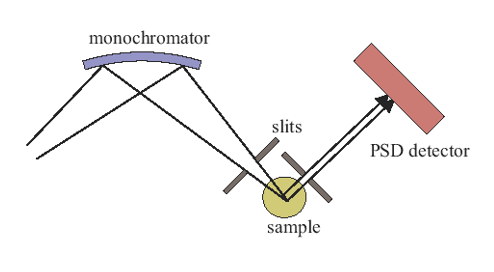
\includegraphics[width=0.6\textwidth]{JS4_difraktometr.png}
	\captionof{figure}{Fokusující difraktometr \label{obr:JS4_neutrina8}}		
\end{center}

Maloúhlový neutronový rozptyl se používá na určování struktur o velikosti $1 - 1000 ~\mathrm{nm}$. Je citlivý na lehké prvky. Zkoumat materiály můžeme v trhačce nebo pícce. Dále můžeme měřit mřížkové konstanty polykrystalických struktur, dále můžeme měřit mikro a makro deformace (studium různých typů ocelí...). Měřit se dají i anizotropie směrů zrn v polykrystalických strukturách - ovlivňuje pevnost a další vlastnosti. Využívá se nepružného neutronového rozptylu.

\subsection{Tříštivé (spalační) reakce jako intenzivní zdroj neutronů}

Využívají se reakce protonu s vysokou energií ($> 100 ~\mathrm{MeV}$) s jádry. Je to velmi intenzivní zdroj neutronů, tím lze dosáhnout až $10^6 ~\mathrm{n/cm^2 \cdotp s}$. Přesně tyto vlastnosti potřebujeme pro efektivní transmutaci (jaderná přeměna, při níž dochází ke změně složení atomového jádra). 

Máme tři etapy tříštivých reakcí:
\begin{itemize}
	\item Vnitrojaderná kaskáda - nalétávající proton vyráží v nukleon-nukleonových srážkách nukleony s vysokou energií, de Broglieho vlnová délka je srovnatelná s velikostí nukleonu $\Rightarrow$ \quotedblbase nukleonový kulečník\textquotedblright ~(relativistické energie)
	\item předrovnovážná emise - výlet nukleonů s vyšší energií z jádra ještě před nastolením tepelné rovnováhy, de Broglieho vlnová délka větší než rozměr nukleonu, energie nejsou relativistické, více pravděpodobné je, že z jádra vylétávají neutrony (nabité částice musí navíc překonat Coulombickou bariéru)
	\item vypařování neutronů nebo štěpení jádra - jádro v tepelné rovnováze se zbavuje přebytečné energie vypařováním neutronů (z vysoce excitovaného jádra) s energií okolo $5 ~\mathrm{MeV}$. Neutrony jsou vypařovány i štěpnými produkty. 
\end{itemize}

Vysokoenergetické neutrony vzniklé v etapě vnitrojaderné kaskády mohou způsobit další tříštivou reakci. Vzniká tak hadronová sprška. 

\subsection{Účinné průřezy pro ADTT (Accelerator Driven Transmutation Technologies) systémy a astrofyziku}

ADS  (Accelerator Driven Systems) jsou systémy sestávající se ze tří hlavních komponentů: urychlovače částic (zejména protonů), terčíku pro spalační (tříštivou) reakci, produkujícího vnější zdroj neutronů, a podkryticky uspořádaného reaktoru, umožňujícího štěpnou reakci. Paprsek iontů je zaměřen na terčík, který je umístěn v centru aktivní zóny. Interakcemi mezi urychlenými částicemi a terčíkem z těžkého kovu se generují neutrony, které udržují štěpnou reakci v reaktoru.

První možností, pro kterou mohou být využity je definitivní izotopická likvidace plutonia, vzniklého hlavně při demontážích zbraňového plutonia zejména v zemích bývalého SSSR, namísto jeho oddělení od životního prostředí (např. trvalým kontrolovatelným uložením), a tak předejít jeho zneužití. Navíc štěpitelné izotopy plutonia představují velký energetický potenciál.  Druhou možností je transmutace izotopů s \quotedblbase rozumným\textquotedblright ~účinným průřezem pro záchyt (absorpci) neutronů. To se ve velké míře týká jak aktinidů, tak i převážné části dlouhodobých štěpných produktů. Transmutační technologie nemohou vyřešit problémy nakládání s vyhořelým palivem \quotedblbase beze zbytku\textquotedblright. 

Zařízení n-TOF v CERNu (Neutron Time of Flight) byl postaven, aby studoval interakce neutronu s jádry pro neutronové energie od $\mathrm{meV}$ až do několika  $\mathrm{GeV}$. Široké spektrum energie a vysoká intenzita svazku neutronů produkované na n-TOF se používá k přesným měřením procesů, které jsou spojené s neutrony.

n-TOF se skládá z:
\begin{itemize}
	\item protonový svazek: $E_p = 20 ~\mathrm{GeV}$, $\Delta t = 7 ~\mathrm{ns}$ (šířka pulzu) , $I = 7 \cdotp 10^{12}$ protonů, $f = 0,8 ~\mathrm{Hz}$
	\item olověný terč - tříštivé reakce
	\item dostaneme neutronový svazek: $300 n/p, E_n = 0,1 ~\mathrm{eV} - 250 ~\mathrm{MeV}$
\end{itemize}
Neutronový zdroj je vzdálený 185 $\mathrm{m}$, intenzita je $10^5$ n/pulz/energetický řád. Má speciální kolimaci a moderaci pro různé režimy práce. Neutronový svazek má $FWHM = 11,8 ~\mathrm{mm}$. 

Měření s n-TOF: různé typy detektorů částic a fotonů, velmi přesná měření ve velmi širokém rozmezí energií, transmisní měření.

\subsection{Studium reakce ($n, \gamma$) na $^{151}$Sm}

\begin{itemize}
	\item poločas rozpadu 93 let - je součástí odpadu jaderných elektráren
	\item důležitý článek řetězce produkce vzácných zemin
	\item patří mezi přechodové prvky
\end{itemize}

Neutrony mají energii od $0,6 ~\mathrm{eV}$ do $1 ~\mathrm{MeV}$. Detekuje se $\gamma$ pomocí $C_6 D_6$ scintilátoru (malá citlivost na neutrony). Přesnost měření je $6 \%$.


\subsection{Produkce neutronů v tříštivých reakcích a srážkách protonů a těžkých iontů}

\begin{itemize}
	\item Příklad měření produkce neutronů v tříštivých reakcích na tenkých terčích:
	\begin{itemize}
		\item použit svazek protonů z cyklotronu v SIN (Švýcarsko) - puls 200 $\mathrm{ps}$
		\item tenké terče
		\item díry ($d = 4 ~\mathrm{cm}$) v 20 $\mathrm{cm}$ železa $\rightarrow$ úzce kolimovaný svazek neutronů do úhlů $30^{\circ}, 90^{\circ}, 150^{\circ}$ (aby nebyl vliv rozptylu)
		\item vzdálenost terče od detektoru je 1,3 $\mathrm{m}$
		\item NE213 - neutronový detektor (plastikový)
		\item NE102A - veto detektor - potlačení nabitých částic (ale neutrony tu interagovat nesmí)
	\end{itemize}
   \item Měření produkce neutronů v tříštivých reakcích do nulového úhlu
   \begin{itemize}
   	\item protonový svazek LAMPF (USA) $E = 800 ~\mathrm{MeV}$
   	\item důležité materiály jsou Al, Ti, Cu, W, Pb, U
   	\item odklonění svazku nabitých protonů a dalších částic magnetem
   	\item konvertorem je tekutý vodík - 0,93 $\mathrm{g/cm^2}$
   	\item výběr jen dopředných protonů vznikajících ve srážkách neutronů (čelní srážky $\rightarrow$ předaná veškerá energie neutronu)
   	\item spektrometr: 4 mnohodrátkové proporciální komory, 2 před a 2 za magnetem (určení hybnosti $\Rightarrow$ na základě toho určíme energii původního neutronu)
   	\item Problémy:
   	\begin{itemize}
   		\item nepružné procesy v konvertoru $n + p \rightarrow p + n + \pi^0 , n + p \rightarrow p +p + \pi^- $
   		\item vznik jiných částic $ n + p \rightarrow d + \pi^0 , n + p \rightarrow d + \gamma$
   		\item pozadí částic vznikajících jinde 
   		\item přesnost znalosti účinného průřezu rozptylu $n - p$ jako funkci energie 
   	\end{itemize}
   \item řada dalších experimentů studujících produkci neutronů v tříštivých reakcích při srážkách těžkých iontů
   \item Podobně se produkují neutrony i na těžkých terčích
   \item je zapotřebí získat data o pravděpodobnostech reakcí a produkci neutronů (i v medicíně, nepotřebujeme přímo neutrony, ale informace o nich potřebujeme, protože můžou vznikat v reakcích)
   \end{itemize}
   \item Měření produkce neutronů na tlustých terčích nebo složitějších sestavách
   \begin{itemize}
   	\item Příklad: sestava \quotedblbase Energy plus transmutation\textquotedblright ~v SÚJV Dubna
   	\item Účel: získat data o produkci a transportu neutronů pro testování simulačních programů
   	\item určování toku a spektra neutronů aktivační metodou
   	\end{itemize}
\end{itemize}

\subsection{Získaná experimentální data}

\begin{itemize}
	\item Měřená data - počet produkovaných jader v aktivačním vzorku normovaný na jeden proton a gram vzorku $\rightarrow$ taková to data lze přímo srovnávat se simulacemi
\end{itemize}

\chapter{Spektroskopie neutrin}

\section{Interakce neutrin}

Neutrina interagují pouze slabou interakcí. Slabá interakce je zprostředkována výměnou intermediálních bosonů:
\begin{itemize}
	\item $Z^0$ - neutrální proudy (byly potvrzeny na experimentu GARGAMEL v Cernu - v bublinové komoře)
	\item $W^+, W^-$ - nabité proudy
\end{itemize}

\begin{center}
	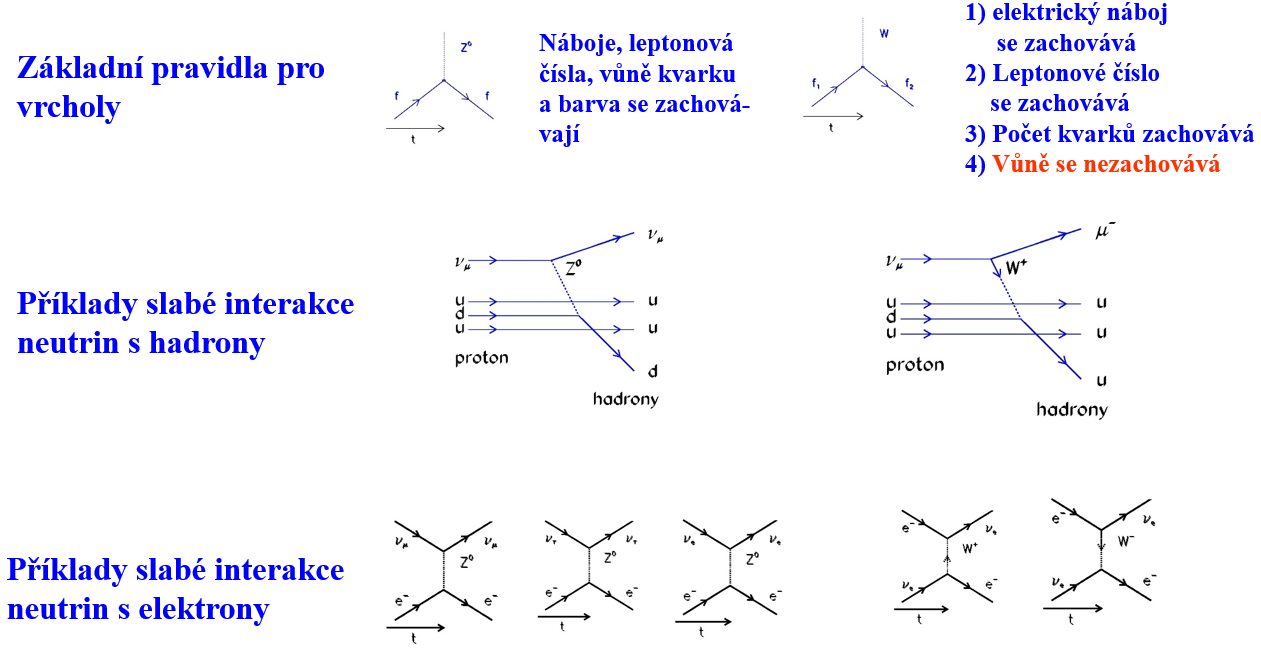
\includegraphics[width=1\textwidth]{JS4_neutrina.png}
	\captionof{figure}{Slabá interakce neutrin \label{obr:JS4_neutrina}}		
\end{center}

\begin{center}
	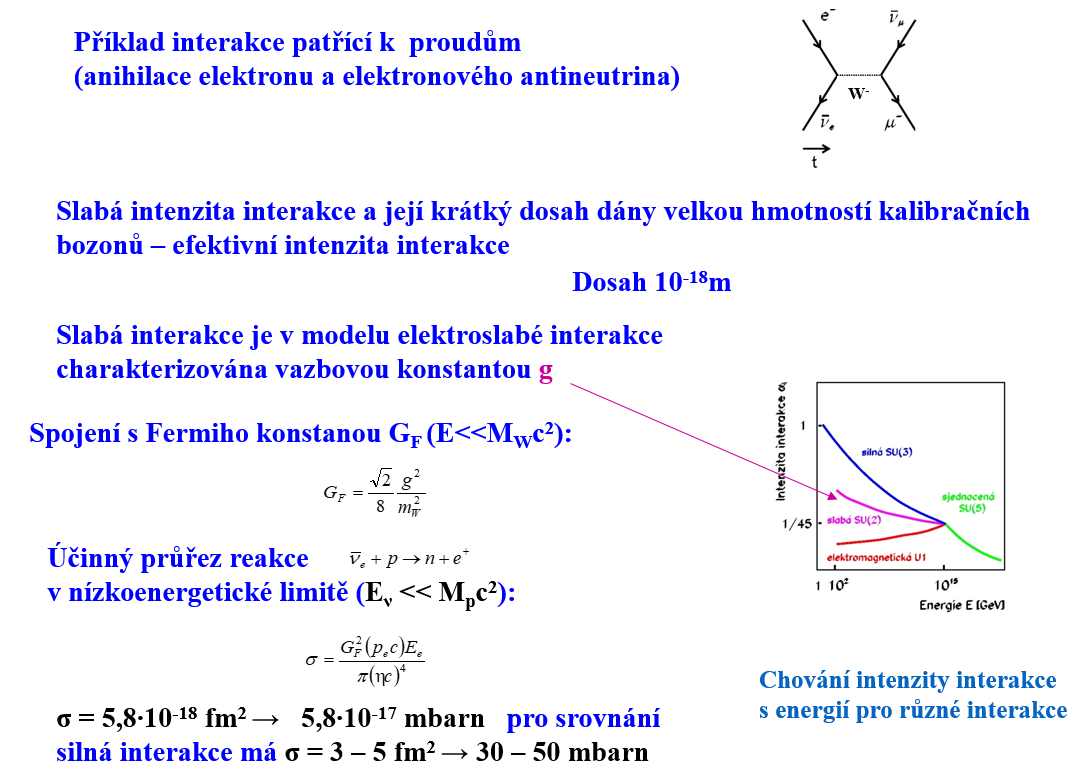
\includegraphics[width=1\textwidth]{JS4_neutrina2.png}
	\captionof{figure}{Slabá interakce neutrin \label{obr:JS4_neutrina2}}		
\end{center}

První detekce neutrin byla provedena v roce 1956 na reaktorech. V reakci $\overline{\nu _e} + p \rightarrow n + e^+$ jsou $e^+$ identifikovány pomocí anihilace v detektoru $\gamma$ záření. Neutrony detekujeme pomocí radiačního záchytu na $Cd$ (přidáme ho to vody). Pomocí záchytu vznikne $Cd^*$, které následně deexcituje a vznikne tak sprška $\gamma$ záření, které detekujeme ve stejném detektoru $\gamma$. 

\subsection{Detekční metody}

Než se budeme věnovat konkrétním detektorům, podívejme se, jaké jsou možnosti interakce neutrin s hmotou. První se bude týkat interakce elektronového neutrina či antineutrina s jádrem. V případě, že elektronové neutrino zasáhne jádro, může v něm přeměnit neutron na proton a vyprodukovat elektron. Celkový počet nukleonů se tím sice nezmění, ale jádro již bude přináležet prvku s počtem protonů o jedničku větším než před srážkou. Při podobné situaci, ale v případě kdy s jádrem interaguje elektronové antineutrino, dochází k snížení protonového čísla, protože se jeden z protonů přemění na neutron za vzniku pozitronu. Tato reakce se často označuje jako inverzní rozpad beta. V obou případech k přeměně jádra dochází jedině tehdy, jestliže má neutrino nebo antineutrino dostatek energie, aby ji způsobilo. Většinou se jedná o reakce určené k detekci neutrin s relativně nízkou energií a pro zjištění jestli proběhly, se identifikuje vzniklé jádro, elektron nebo pozitron (často pomocí své anihilace).

V extrémním případě, kdy je energeticky možný samovolný rozpad beta jádra za vzniku elektronu nebo pozitronu, může způsobit jeho rozpad i reakce s neutrinem, které má extrémně nízkou energii. Například, pokud budeme mít jádro tritia a bude s ním interagovat elektronové neutrino i s extrémně malou energií, proběhne jeho přeměna na izotop helia s třemi nukleony za vzniku elektronu. Jde tedy o proces, obdobný beta rozpadu tritia, jen v něm nevzniká antineutrino. Všechnu energii tak odnáší vzniklé jádro a elektron. Na počátku je jádro tritia v klidu a u neutrina jsme předpokládaly zanedbatelně malou energii. Elektron tak má v takovém případě vždy stejnou energii a rovnou maximální možné energii elektronu v rozpadu tritia zvýšenou o dvojnásobek klidové energie neutrina (ta je ovšem extrémně malá). Nemusí se totiž vytvářet antineutrino jako v rozpadu tritia, ale naopak, do reakce neutrino vstupuje z vnějšku. Tyto reakce jsou velice zajímavé, jsou totiž jednou z mála možností, jak by se v budoucnu mohly přímo detekovat reliktní neutrina, tedy alespoň reliktní elektronová neutrina a antineutrina.

Další možností je produkce různých leptonů (elektronů, mionů nebo tauonů) v interakcích s jádry a elektrony. V tomto případě se jedná o možnost detekce neutrin s vyššími energiemi, protože zvláště reakce, při kterých vzniká těžký mion a ještě těžší tauon, potřebují značně vysokou energii pro jejich vytvoření. Při velmi vysokých energiích neutrin, které se uplatňují například při studiu neutrin, které jsou součástí primárního vysokoenergetického kosmického záření, se v primárních i sekundárních reakcích s jádry uvolňuje hodně energie a může se produkovat velké množství dalších částic (produkují se tzv. hadronové a elektromagnetické spršky). Vznikající nabité částice můžeme detekovat pomocí jejich ionizace v materiálu detektoru. Částice s dostatečně vysokou energií, které se pohybují rychlostí větší než je rychlost světla v materiálu detektoru, pak mohou být detekovány pomocí Čerenkovova záření.

Pro detekci neutrin s velmi nízkou energií by se mohl využít pružný rozptyl na elektronech nebo pružný rozptyl na jádrech. Vzhledem k tomu, že neutrino může předat objektu, na kterém se pružně odrazí, tím více energie, čím je objekt lehčí, je mnohem výhodnější využívat pružný rozptyl na elektronech. I při něm však předává neutrino jen část své energie. Tuto reakci využívá pro detekci neutrin například detektor SuperKamiokande. Rozptyl elektronových neutrin na elektronech je mnohem pravděpodobnější než rozptyl dalších typů neutrin. Pokud chceme detekovat neutrina s velmi malou energií, narazíme na závažnou překážku. Energie elektronů či jader, na kterých se neutrino rozptyluje, je ještě daleko menší. Je pak problém s vytvořením detektoru, který by tento jev využíval. Zatím existují návrhy experimentů využívajících velmi přesnou nízkoenergetickou kalorimetrii.

\begin{itemize}
	\item Obrácený rozpad $\beta$:
	\begin{equation}
	\overline{\nu _e} + p \rightarrow n + e^+
	\end{equation}
	proton se neexcituje $\rightarrow$ lze určit energii neutrina: $E_{\nu} = E_e + E_{od} + (E_n - E_p)$
	\begin{itemize}
		\item Záchyt na těžkých jádrech: 
		\begin{equation}
		\overline{\nu _e} + (Z,N) \rightarrow e^+ + (Z-1,N+1)
		\end{equation}
		\begin{equation}
		\nu_e + (Z,N) \rightarrow e^- + (Z+1,N-1)
		\end{equation}
		$\Rightarrow$ detekce pouze elektronových neutrin a antineutrin
	\end{itemize}
	\item Produkce $e^{\pm}, \mu^{\pm}, \tau^{\pm}$: následná detekce nabitých leptonů a určení jejich energie $\Rightarrow$ detekce všech druhů neutrin a antineutrin
	\item Rozptyl na elektronech: následná detekce odražených elektronů $\Rightarrow$ detekce všech druhů neutrin a antineutrin - možnost detekce neutrin i s velmi nízkými energiemi
	\item Rozptyl na jádrech: následná detekce odražených jader $\Rightarrow$ detekce všech druhů neutrin
\end{itemize}
	

\section{Detektory neutrin}

Přejděme teď ke konkrétním typům detektorů, které využívají popsané způsoby interakce neutrin s hmotou. Jen je třeba ještě zdůraznit, že všechny typy neutrinových detektorů jsou díky malé pravděpodobnosti reakcí neutrin velice citlivé na pozadí. Proto se musí umisťovat do podzemí a je třeba co nejvíce potlačit úroveň přirozené radioaktivity v místě detektoru.

Obecné charakteristiky:
\begin{itemize}
	\item velmi malé průřezy interakcí  $\rightarrow$ velmi velké objemy detektorů
	\item velmi efektivní stínění $\rightarrow$ podzemní detektory, podvodní, pod ledem 
\end{itemize}

Typy detektorů:
\begin{itemize}
	\item Radiochemické detektory
	\item Detektory Čerenkovova záření
	\item Scintilační detektory
	\item Detektory na základě rozptylu neutrin na elektronech
\end{itemize}

\subsection{Radiochemické detektory}

První typ detektorů, na který se podrobněji podíváme, jsou detektory radiochemické. Jsou vhodné pro neutrina s nižší energií. V tomto případě se využívá reakce neutrina či antinenutrina se stabilním jádrem, při které vznikne jádro radioaktivní a elektron nebo pozitron. Pokud vybereme vhodnou reakci, abychom vzniklá radioaktivní jádra dokázali efektivně separovat, identifikovat a určit jejich počet, můžeme je využít pro měření intenzity toku elektronových neutrin (antineutrin) v daném místě. Hodnotu energie detekovaných neutrin neurčíme a můžeme odhalit pouze neutrina, jejichž energie je vyšší než minimální potřebná pro uskutečnění dané reakce (prahová energie). Problémem je, že reakce neutrin jsou zřídkavá a tak se produkují pouze jednotlivé radioaktivní jádra. Proto velice účinná musí být jednak chemická separace vzniklých jader ale i následná detekce jejich rozpadu. Proto se u současných detektorů radioaktivní jádra převádí do plynné formy a stávají se součástí plynné náplně proporcionálních čítačů, které detekují radioaktivitu. Samotné měření má dva cykly. V prvním probíhá delší dobu expozice, kdy náplň v nádrži detektoru zachycuje neutrina a vznikají radioaktivní jádra (nabírání dat). Po skončení expozice následuje extrakce radioaktivních jader z náplně nádrže a měření jejich radioaktivity. Po extrakci lze zahájit novou expozici (radiochemická analýza). Nevýhodou tohoto typu detektorů je, že detekují pouze elektronová neutrina, případně někdy v budoucnu budou i antineutrina. Jak už bylo řečeno, nelze určit energii neutrin, získáme pouze informaci o jejich globálním počtu, který detektor v celém průběhu expozice zachytil. Výhodou je možnost detekce neutrin s velmi nízkou energií a velmi vysoká citlivost těchto detektorů. Z detektoru, který obsahuje 1030 atomů, může být získáno a spolehlivě identifikováno i jen deset atomů produkovaných v reakcích neutrin.

Využívají se například reakce:
\begin{itemize}
	\item $\nu _e + ^{37}Cl \rightarrow ^{37}Ar + e^-$
	\item $\nu_e + ^{71}Ga \rightarrow ^{71}Ge + e^-$
\end{itemize}

Takový to detektor využívají např. \textbf{experiment GALLEX v Gran Sasso}, který byl druhý, který se zabýval detekcí neutrin pomocí galiového detektoru. Nebo \textbf{chlorový experiment} R. Davise (detekoval sluneční neutrina).

\subsection{Detektory vyplněné vodou a využívající detekci Čerenkovova záření}

Dalším typem detektorů, které zasáhly do řešení problému s deficitem slunečních neutrin, jsou detektory využívající pro jejich detekci velký vodní bazén. Podrobněji si popišme japonský detektor Kamiokande, který je umístěn v podzemí, v hloubce zhruba jednoho kilometru pod povrchem. Původně hledalo toto zařízení rozpady protonu. V roce 1987 úspěšně zachytilo neutrina ze supernovy a bylo rozhodnuto, že se bude věnovat detekci neutrin ze Slunce. Při práci v oblasti nízkých energií, které neutrina ze Slunce mají, se využíval pružný rozptyl neutrin na elektronech, při kterém se předala elektronu dostatečná energie k tomu, aby jeho rychlost byla větší než rychlost světla ve vodě. Takový elektron vyzařuje tzv. Čerenkovovo světlo. Vzniklé záblesky světla se zaznamenávají pomocí velkého počtu fotonásobičů umístěných okolo vodního bazénu. Z těch důvodů bylo potřeba co nejpečlivěji vyčistit vodu v bazénu detektoru od radioaktivních příměsí (jednou z hlavních byl izotop radonu $^{222}$Rn přítomný ve vzduchu). Zároveň se k identifikaci reakcí způsobených neutriny využívala jen vnitřní část detektoru. Vnější část sloužila k identifikaci elektronů z pozadí, které přilétly z vně detektoru. Detektor určí ze směru, do kterého je vyzařováno Čerenkovovo záření, směr letu elektronu a ten je dán původním směrem letu neutrina. V principu se na elektronech mohou rozptylovat všechny typy neutrin, ovšem pravděpodobnost tohoto rozptylu v této oblasti energií pro jiné typy, než jsou elektronová neutrina, je zhruba šestkrát nižší. Vznikající Čerenkovovo záření zaznamenávalo 11 000 velkých fotonásobičů. Zároveň se podařilo snížit nejnižší možnou energii detekovaných neutrin z $9 ~\mathrm{MeV}$ na $5 ~\mathrm{MeV}$. Pořád však to stačilo pouze na detekci jen těch nejenergetičtějších neutrin ze Slunce. \textbf{SuperKamiokande} byl první, který využil své možnosti určit směr příchodu neutrin a potvrdil, že přicházejí opravdu ze Slunce.

\begin{itemize}
	\item Výhody: snadno dostupný materiál (voda)
	\item Nevýhody: prahová energie je vyšší než u scintilačních detektorů (dostaneme se s energií níž), jen část energie je předána $e^+ , e^-$.
\end{itemize}	 

\subsection{Detektory využívající těžkou vodu}

V roce 1998 byla dokončena konstrukce detektoru SNO (Sudbury Neutrino Observatory) umístěného v kanadském dole v hloubce přes dva kilometry pod povrchem. Ten měl vnitřní a vnější nádrž. Vnitřní nádrž, která fungovala jako pracovní objem pro detekci neutrin, byla naplněna tisícem tun těžké vody (lehký vodík je v ní nahrazen svým těžším izotopem – deuteriem, složeném z jednoho protonu a jednoho neutronu). Vnější nádrž, která sloužila jako v případě detektoru SuperKamiokande k identifikaci pozadí, měla sedm tisíc tun této normální vody. Během budování detektoru byla extrémní pozornost věnována co nejvyšší čistotě použitých materiálů a co nejnižšímu jejich radioaktivnímu pozadí. K identifikaci reakcí bylo opět využíváno Čerenkovovo záření a k jeho zachycení sloužilo okolo 9500 velkých fotonásobičů.

V oblasti energií slunečních neutrin dochází v tomto typu neutrinového detektoru k třem typům reakcí. Stejně jako v případě detektoru SuperKamiokande dochází k rozptylu neutrin na elektronech. Tento proces je pro elektronová neutrina zhruba šestkrát pravděpodobnější než pro ostatní typy neutrin. Dochází však k dvěma novým typům procesů. Elektronové neutrino může přeměnit neutron v deuteronu na proton za vzniku elektronu. I v tomto případě může být jako v předchozím elektron identifikován pomocí Čerenkovova záření, které elektron s rychlostí přesahující rychlost světla v těžké vodě vyzařuje. Nejdůležitější je však třetí typ reakcí. Ten produkuje všechny typy neutrin se stejnou pravděpodobností. Jde o rozbití deuteronu na neutron a proton (nepružný rozptyl).

\begin{center}
	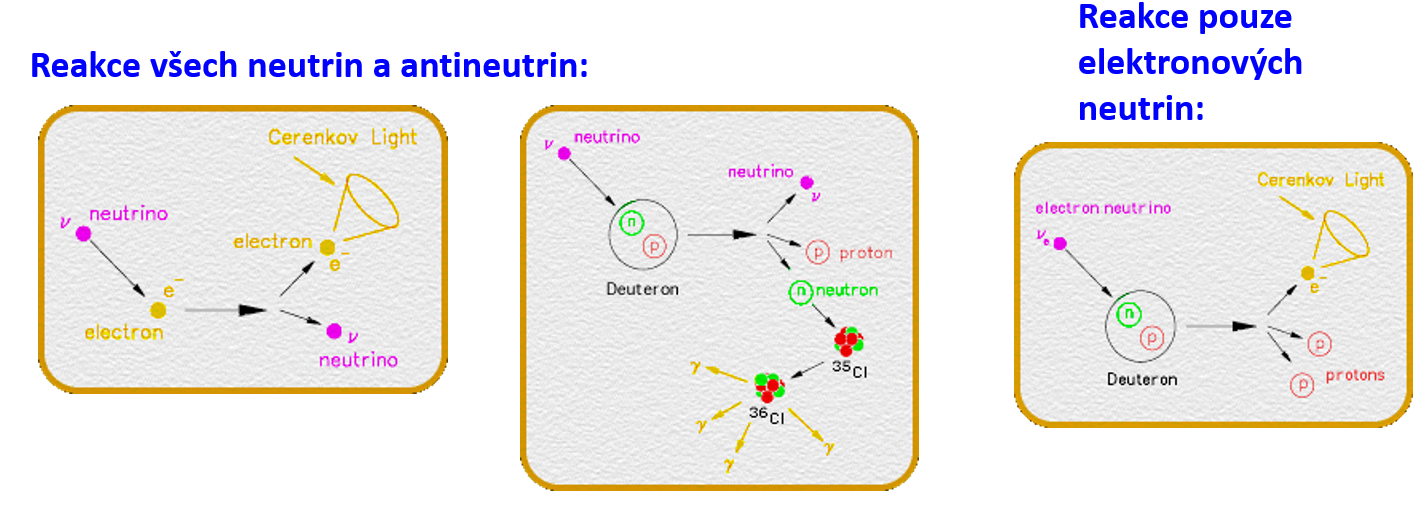
\includegraphics[width=1.05\textwidth]{JS4_reakceneutrin.png}
	\captionof{figure}{Reakce neutrin a antineutrin \label{obr:JS4_neutrina4}}		
\end{center}

\subsection{Detektory využívající scintilační materiál}

Snaha o zachycení neutrin s co nejnižší energií vedla k využití scintilačních kapalných detektorů. Aby měl elektron po rozptylu neutrina na něm dostatečnou energii a rychlost, aby vyzařoval Čerenkovovo záření, musí mít neutrino dostatečně velkou energii. Ionizovat však může elektron i s energií daleko nižší. Pokud má látka, kterou ionizující elektron prolétá, schopnost vytvářet scintilační světlo, můžeme toto světlo zaznamenat fotonásobiči podobně jako světlo Čerenkovo. Tím lze získat informaci o dráze elektronu a neutrina, které se na něm rozptýlilo.

Stejným typem detektoru je i japonský \textbf{KamLAND}, který je umístěn ve stejném místě jako SuperKamiokande. Jeho pracovní vnitřní objem obsahuje téměř tisíc tun organické tekutiny, na kterou se dívá téměř dva tisíce fotonásobičů.

Neutrinový detektor \textbf{Borexino} byl vybudován v evropské podzemní laboratoři Gran Sasso. Využívá tři sta tun super čistého organického kapalného scintilátoru, na který se dívá 2200 velkých fotonásobičů. Stínění zase zajišťuje vnější vrstva velmi čisté vody.

\subsection{Detektory vysokoenergetických neutrin}

Doposud jsme se snažili zachytit neutrina s co nejnižší energií. Nyní se vydáme na cestu opačným směrem energetické stupnice. V případě vysokých energií neutrin je možno několik typů reakcí, při kterých vznikají různé typy nabitých částic.

Jednou možností je vznik nabitých leptonů s vysokou energií - elektronu, mionu, nebo tauonu. Ty pak mají různé osudy. Elektron v hmotném prostředí produkuje brzdné záření - fotony gama. Pokud i ty mají vysokou energii, produkují páry elektronu a pozitronu, ty mohou opět produkovat brzdné záření. Dostáváme tak spršku fotonů záření gama, elektronů a pozitronů – elektromagnetickou spršku. V případě vzniku tauonu se tento rychle rozpadne. Jeho poločas rozpadu je v řádu 10-13 s a za tu dobu nestihne uletět dráhu ani sto mikrometrů. Produkty jeho rozpadu mohou být buď mion, nebo elektron, případně nabité částice, které interagují silnou interakcí (hlavně mezony).

Druhou možností je vznik nabitých silně interagujících částic (ty se označují jako hadrony), ty pak mohou při pohybu materiálem produkovat stále další takové částice. Dostáváme tak tzv. hadronovou spršku. V obou případech dostaneme nabité částice pohybující se rychlostmi, které překračují rychlost světla v daném prostředí. Ty mohou jednak vyrážet elektrony z atomů prostředí (ionizovat) a také produkovat Čerenkovovo záření. Oba tyto jevy se tak dají využít k detekci těchto částic a tím i původního neutrina.

Řada detektorů vysokoenergetických neutrin je složena z tlusté vrstvy materiálu, která slouží k interakci neutrina a rozvoji spršky nabitých částic a detektorů, které slouží k detekci těchto částic pomocí ionizace nebo Čerenkovova světla.

\subsection{Detektor ANTARES ve Středomoří}

My se blíže podíváme na dva detektory kosmických neutrin s extrémně vysokými energiemi. Hustota takových neutrin je hrozně malá. Proto potřebujeme detektory o extrémně velkém objemu. První, který si rozebereme, využívá jako detektor velký objem vody ve středozemním moři. Čerenkovové záření vznikající při pohybu nabitých částic, vzniklých při interakci neutrina, je detekováno pomocí fotonásobičů. 

Důležité je, že ze směru, do kterého je vyzařováno Čerenkovovo záření, lze určit, jakým směrem se částice, které je vyzařují, pohybují. V případě detekce neutrin se vybírají případy, kdy částice letí ve směru ode dna k hladině. Důvodem je, že částice kosmického záření, hlavně miony, pronikají hluboko pod hladinu a vytvářejí tak pozadí, ve kterém se daleko menší počet případů vzniklých z interakce neutrin ztratí. Ze směru od středu Země však žádné miony kosmického záření nepřilétají.

\subsection{AMANDA - Neutrinový detektor pod ledem, IceCube}

Další podobný typ detektoru se postupně buduje v Antarktidě. Tentokrát se využívá místo vody led. Do děr, které vzniknou roztavením ledu, se spustí kabel, na kterém jsou umístěny fotonásobiče. Ty po zamrznutí vody v díře detekují, jako v případě předchozího experimentu, Čerenkovovo záření, které produkují nabité částice vzniklé reakcí kosmického neutrina. Opět je třeba využívat pouze případy spršek nabitých částic, které letí směrem z hlubin Země k povrchu. V opačném směru totiž pozoruje Ice Cube na každý mion pocházející z neutrina milión mionů pocházejících z interakcí nabitých částic primárního kosmického záření. 

\subsection{Rozptyl neutrina na elektronu}

Tímto způsobem můžeme detekovat i neutrina s velmi nízkou energií. K potlačení šumu se používá tekuté nebo supratekuté hélium (při velmi nízkých teplotách - $10 ~\mathrm{mK}$). Jelikož máme malou energii neutrin $\sim ~\mathrm{keV}$, máme i malou energii odražených elektronů. Probíhat může ionizace, scintilace, vznikají pak fonony, rotony, které jsou následně zachycovány safírovou či křemíkovou destičkou - absorbátor $\rightarrow$ kontrola teploty. Kontrola teploty je prováděna pomocí \textbf{Mikrokalorimetrů} (dokážou zaznamenat velmi malé změny teploty). Zachycení \quotedblbase driftujících\textquotedblright ~elektronů - \quotedblbase elektronová bublina\textquotedblright ~v supratekuté supravodivé kapalině se pohybuje kontrolovaně v elektrickém poli.

Např. experiment \textbf{HERON}.

\section{Aplikace spektroskopie neutrin}

\begin{itemize}
	\item Detekce slunečních neutrin
	\item Detekce neutrin ze supernov
	\item Detekce neutrin z kosmického záření
	\item Studium oscilace neutrin
	\item Detekce neutrin z nitra Země
	\item detekce reliktních neutrin
\end{itemize}

\subsection{Studium slunečních neutrin}

V průběhu $pp$ i CNO cyklu se produkuje velké množství elektronových neutrin
\begin{equation}
4p \rightarrow ^{4}He + 2 e^+ + 2 \nu_e.
\end{equation}

Dosavadní informace:
\begin{itemize}
	\item neutrina ve Slunci opravdu vznikají
	\item významný rozdíl mezi předpověďmi a pozorováními $\rightarrow$ signál nové fyziky (oscilace neutrin)
\end{itemize}

Budoucí informace z neutrin:
\begin{itemize}
	\item přesný rozměr centrální oblasti Slunce, kde probíhají termojaderné reakce
	\item současný obraz centra Slunce (fotony putují z jádra ven velmi dlouho)
	\item teplota centrálních oblastí Slunce
	\item poměry mezi zastoupením různých typů fúzních reakcí
\end{itemize}

\subsection{Studium neutrin ze supernov}

Konečným stádiem hmotné hvězdy je její kolaps a výbuch supernovy. Velká část energie se uvolní ve formě neutrin ve dvou fázích:
\begin{itemize}
	\item počátek - při vzniku neutronů elektronových záchytek vznikají pouze elektronová neutrina: $p + e^- \rightarrow n + \nu_e$
	\item všechny druhy neutrin a antineutrin se statistickým zastoupením (1/6 na jeden typ) se střední energií $10 - 15 ~\mathrm{MeV}$. Energetické spektrum má Fermiho rozložení $kT \approx 3-6 ~\mathrm{MeV}$
\end{itemize}

Supernova SN 1987A je první a prozatím i poslední, ze které se nám podařilo zachytit neutrina (zdroj NASA). Její vzdálenost je 150 000 světelných let.

Dosavadní informace:
\begin{itemize}
	\item potvrzení vzniku neutrin
	\item řádový souhlas s předpoklady
	\item blízkost rychlosti neutrin rychlosti světla, omezení na klidovou hmotnost neutrina
	\item určení limity pro dobu života neutrina
\end{itemize}

Možné budoucí informace (čekáme na blízkou supernovu):
\begin{itemize}
	\item potvrzení modelů výbuchu supernovy
	\item chování horké a velmi stlačené hmoty
	\item pozorování supernov zastíněných galaktickou hmotou
\end{itemize}

\subsection{Neutrina z kosmického záření}

Primární složku tvoří částice s vysokou energií (až $\sim 10^{11} ~\mathrm{GeV}$ - dnešní urychlovače $\sim 10^{4} ~\mathrm{GeV}$), největší část tvoří protony a jádra. Část tvoří i neutrina a antineutrina $\nu_e, \nu_{\mu}, \nu_{\tau}$. Částice mají izotropní rozložení, tj. přicházejí ze všech směrů. Původ primárního kosmického záření: vzdálenější nerozlišitelné zdroje (supernovy, aktivní jádra galaxií, kolabující objekty ...).

Sekundární složka kosmického záření vzniká při srážkách částic a jader kosmického záření s jádry atmosféry. Při tom vzniká spousta hadronů, mezi nimi je i spousta mezonů $\pi$:
\begin{equation}
\pi^+ \rightarrow \mu^+ + \nu_{\mu} , ~~~~~ kde ~~~~~~ \mu^+ \rightarrow e^+  + \nu_e + \overline{\nu_{\mu}}
\end{equation}
\begin{equation}
\pi^- \rightarrow \mu^- + \overline{\nu_{\mu}}, ~~~~~~  kde ~~~~~ \mu^- \rightarrow e^- + \overline{\nu_e} + \nu_{\mu}
\end{equation}

Tyto reakce jsou intenzivním zdrojem neutrin a antineutrin $\nu_{\mu}$ a $\nu_e$. Poměr mezi počtem $\nu_{\mu}$ a $\nu_e$ je $R(\nu_{\mu} /\nu_e)= 2$. Zároveň jsou tyto reakce intenzivním zdrojem mionů.

Možné budoucí informace:
\begin{itemize}
	\item hledání kosmických neutrin, která by byla spojena s největšími ohňostroji ve vesmíru - zábleskovými zdroji $\gamma$
	\item neutrina vznikající v rozpadech a interakcích částic temné hmoty. Tyto částice, nejčastěji se uvažují supersymetrická neutralina, by se v naší Sluneční soustavě mohly díky gravitační přitažlivosti koncentrovat ve Slunci a produkovat neutrina a antineutrina vysokých energií ve svých anihilačních procesech
	\item dráha neutrin není ovlivněna magnetickými poli a nejsou pohlcována 
	\item odhalení podstaty i nepředpokládaných kosmických jevů
\end{itemize}
	
Sekundární kosmická neutrina vznikající v atmosféře se detekují a studují běžně a jejich analýza přinesla řadu fundamentálních informací hlavně o oscilacích neutrin. Na detekci primárních kosmických neutrin citlivost současných detekčních systémů zatím nestačí. Ovšem pokrok, který čekáme v nejbližší době u experimentů ANTARES a Ice Cube, by mohl přinést zásadní zlom v této oblasti. Vysokoenergetická kosmická neutrina by nám pak mohla přinést řadu důležitých informací o těch nejenergetičtějších procesech ve vesmíru.

Výsledky z detektoru AMANDA - spektrum neutrin odpovídá předpovědím pro atmosférická neutrina. Rozložení směrů, ze kterých přišly jednotlivá neutrina, má náhodné rozdělení. Bodové zdroje nebyly nalezeny, nebyly nalezeny korelace se zábleskovými zdroji $\gamma$. 	

\subsection{Studium oscilací neutrin}

Vlnová funkce neutrina je směs různých stavů ($\nu_e, \nu_{\mu}, \nu_{\tau}$). Jako příklad uvedeme oscilace $\overline{\nu_{\mu}}$ a $\overline{\nu_e}$:
\begin{equation}
\left( {\begin{array}{c}
	\overline{\nu_e}   \\
	\overline{\nu_{\mu}}  \\
	\end{array} } \right)
\left({\begin{array}{cc}
\cos \Theta & \sin \Theta \\
	- \sin \Theta & \cos \Theta \\
	\end{array} } \right)
\left( {\begin{array}{c}
	\nu_1   \\
	\nu_2  \\
	\end{array} } \right).
\end{equation} 

Pravděpodobnost přechodu mionového antineutrina v elektronové je:
\begin{equation}
P(\overline{\nu_{\mu}} \rightarrow \overline{\nu_e}) = \sin^2 2\Theta \cdotp \sin ^2 (1,27 \times \Delta m^2 \times L/E_{\nu}),
\end{equation}
kde $\Delta m ^2 = \left| m_{1}^2 - m_{2}^2 \right| [\mathrm{eV^2}]$, $L$ je vzdálenost v metrech $[\mathrm{m}]$ a $E_{\nu}$ je energie neutrina $[\mathrm{MeV}]$. Pravděpodobnost, že ve vzdálenosti $d$ nalezneme $\overline{\nu_{\mu}}$, je $P(\overline{\nu_{\mu}}) $ a $\overline{\nu_e}$ je $P(\overline{\nu_e})$. Toto je vidět na následujícím obrázku.

\begin{center}
	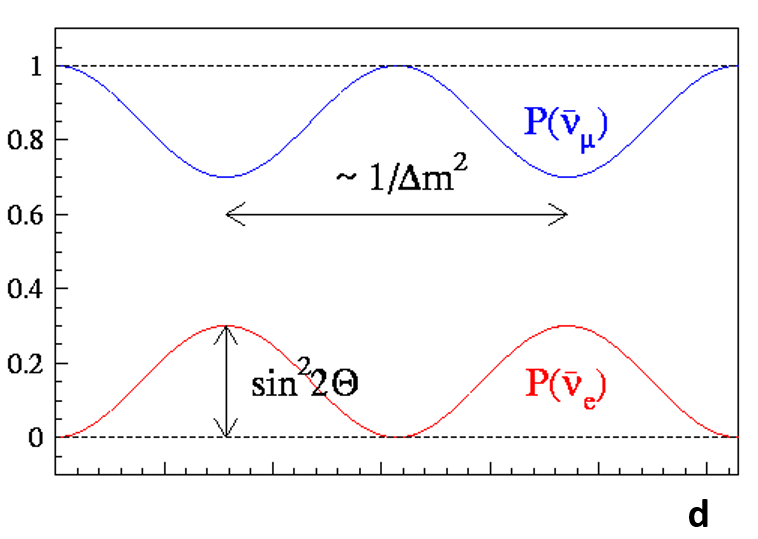
\includegraphics[width=0.6\textwidth]{JS4_slunecni.png}
	\captionof{figure}{Pravděpodobnost, že ve vzdálenosti $d$ nalezneme $\overline{\nu_{\mu}}$, je $P(\overline{\nu_{\mu}}) $ a $\overline{\nu_e}$ je $P(\overline{\nu_e})$ \label{obr:JS4_neutrina5}}		
\end{center}

Oscilace byly pozorovány:
\begin{itemize}
	\item ve slunečních neutrinech (velké vzdálenosti)
	\item v jaderných elektrárnách
	\item v sekundárním kosmickém záření
	\item v urychlovačích - detektorech
\end{itemize}	
	
\subsection{Sluneční neutrina}

Byl odvozen vztah 
\begin{equation}
\Delta m^2 (\nu_e \leftrightarrow \nu_{\mu}) \sim 7(4) \cdotp 10^{-5} ~\mathrm{eV^2}
\end{equation}

\subsection{Měření reaktorových antineutrin}

Díky neutrinům z reaktoru se existenci těchto částic podařilo prokázat. V reaktoru se produkuje velké množství neutronů. Při záchytu neutronu stabilními jádry vznikají jádra, která mají přebytek neutronů. Stejně tak mají přebytek neutronů radioaktivní jádra vznikající při štěpení. Při rozpadech beta neutronů i zmíněných radioaktivních jader s přebytkem neutronů se produkují elektronová antineutrina. Reaktor je tak velmi intenzivním zdrojem elektronových antineutrin. Řada reaktorů se tak využívá nebo plánuje využít pro studium oscilací elektronových antineutrin. Jistým omezením je to, že nelze definovat energii těchto antineutrin, reaktor produkuje antineutrina se spojitým rozložením energií a navíc jejich maximální energie je relativně malá.

Detekce antineutrin 
\begin{equation}
\Delta m^2 (\nu_e \leftrightarrow \nu_{\mu}) \sim 7,9(6) \cdotp 10^{-5} ~\mathrm{eV^2}
\end{equation}

\subsection{Neutrina z urychlovačů}

Pomocí vysokoenergetických reakcí urychlených částic můžeme získávat relativně velmi intenzivní svazky neutrin a antineutrin. Nabité částice vznikající při těchto reakcích lze odklonit pomocí magnetického pole. Ostatní částice interagují daleko více s materiálem a můžeme je tak dostatečně tlustou vrstvou odstínit a získat tak čistý neutrinový svazek.

\subsection{Urychlovač - detektor experiment}

Takovým to experimentem je experiment K2K. Ten pozoroval 108 neutrin, předpovězeno bylo 151(11) neutrin. 

\subsection{Sekundární kosmické záření}

Pro $\nu_{\mu} \leftrightarrow \nu_{\tau}$ máme:
\begin{equation}
\Delta m^2 (\nu_e \leftrightarrow \nu_{\mu}) \sim (1-3) \cdotp 10^{-3} ~\mathrm{eV^2},
\end{equation}
kde $\nu_e$ má izotropní rozdělení, $\nu_{\mu}$ má úbytek.


\subsection{Geoneutrina}

V zemské kůře i nitru je obsaženo značné množství radioaktivních izotopů. Ty se často rozpadají i některou z forem rozpadu beta. Tím dochází k produkci elektronových neutrin a antineutrin. Nejintenzivnějšími zdroji těchto neutrin jsou rozpadové řady začínající u thoria a uranu, tedy jader $^{232}$Th, $^{238}$U a $^{235}$U s poločasy rozpadu $14,1$; $4,5$ a $0,7$ miliard let. Dalším zdrojem je i izotop draslíku $^{40}$K s poločasem rozpadu 1,3 miliardy let. Přesný počet těchto neutrin a rozložení jejich zdrojů a jejich spektrum zatím neznáme, protože neznáme přesné rozložení výskytu radioaktivních izotopů uvnitř Země. Právě naopak, pokud by se nám podařilo vybudovat dostatečně citlivé detektory neutrin, mohly by nám geoneutrina přinést hodně informací o složení zemského nitra.

Projekt KamLAND - studium oscilací antineutrin z reaktorů. Prvním pozorováním zachytil projekt KamLAND $4-40$ geoantineutrin. To odpovídá modelovým představám o množství uranu a thoria v zemské kůře a jádru. 

\subsection{Reliktní neutrina}

Celý náš vesmír je vyplněn reliktními neutriny a antineutriny, které vznikly v průběhu Velkého třesku. Jednotlivé typy neutrin a antineutrin jsou v něm zastoupena rovnoměrně. Ve velmi horkém počátečním stavu vesmíru byly procesy, při kterých při srážkách neutrina a antineutrina vznikají dvojice leptonu a antileptonu a při srážkách leptonu a antileptonu pak vznikají dvojice neutrina a antineutrina, v rovnováze. Pokud však klesla teplota vesmíru tak, že energie neutrin byla nižší než zhruba $1 ~\mathrm{MeV}$ (dvojnásobek klidové energie elektronu), střední volná dráha pro všechny typy neutrin vzroste tak, že už nemohla interagovat s hmotou a pole neutrin a antineutrin se oddělilo od hmoty. Chladnutí neutrin s rozpínáním vesmíru probíhalo nezávisle na ostatní hmotě. V té době, kdy od počátku rozpínání našeho vesmíru uplynula zhruba jedna sekunda, byla teplota hmoty ve vesmíru a i neutrin $3 \cdotp 10^{10} ~\mathrm{K}$.

Reliktní neutrina mají velmi nízkou energii a tak je jejich přímá detekce velmi obtížná.
Jejich existenci se však již podařilo prokázat alespoň nepřímo. Důkaz je založen na tom, že během velmi raných fází vývoje vesmíru, než došlo k popsanému oddělení neutrin od ostatní hmoty, byl jejich podíl na hustotě energie až desítky procent a ovlivňovaly průběh rozpínání našeho vesmíru. Měly tak vliv na průběh prostorové anizotropie v hustotě a energii hmoty v těchto raných fázích vývoje vesmíru a informace o tomto ovlivňování lze najít v průběhu anizotropií v teplotě reliktního elektromagnetického pozadí.



\end{document}